\documentclass[a4paper,11pt]{ltjsarticle}
\usepackage{amsmath,amssymb}
\usepackage{graphicx}
\usepackage{geometry}
\usepackage{longtable}
\usepackage{booktabs}
\usepackage{enumitem}
\usepackage{url}
\usepackage{makecell}
\geometry{margin=25mm}

\title{党勢推移指数プロジェクト 全体設計書}
\author{}
\date{2026年9月}

\begin{document}
\maketitle

\section{概要}

本稿では、政党の党勢(政治的な勢い)の推移を定量化する非公式の定点観測プロジェクトの設計をまとめます。メインコンテンツは、国会(衆参)の選挙と知事・市区町村長の選挙を1本に統合した単一の指数$C_p(T)$(\S2)であり、議会と執行機関を別建てで追跡することはしません。指数の算出コード自体はgitで公開し、算出式・データソースを読者が検証できる状態にすることを設計の前提とします。

当初は「現時点で誰が何を保有しているか」を毎月まるごと積み上げるストック方式で、これだと選挙結果が変わってもどの政党がその枠を持つかが変わるだけで指数の値自体はほとんど動きませんでした。実際に選挙があった選挙イベントだけを対象にするフロー方式へ変更したことで(\ref{sec:rationale}節)、選挙のたびに指数が実際に動く設計になりました。これを受けて、note記事は月1回を目安に更新するスケジュールを目指します。ただしこれは達成を強制される「ノルマ」ではありません——本プロジェクトはあくまで趣味の定点観測であり、義務化するとかえって続かなくなります。あくまで緩い目安として、政治的な主張(「党勢が落ちている/伸びている」等)を検証したくなったタイミングでも随時参照できるデータとして運用します。

\subsection{動機}

発端は、ある政党の党首が党勢の低下を「謀略だ」と主張する一方、支持者が「まだ伸びている」と主張していたからです。実際どちらが正しいのかを客観的に判断できる指標を探しましたが、既存のものはいずれも難がありました。X(旧Twitter)の投稿数はリアルタイム性に優れますが、ネガティブな言及が存在したり自作自演の投稿があったりして、直接的な利用は困難です。また、世論調査は誤差が数\%程度ある上に「支持政党なし」の割合が大きすぎて実質的な政治力を反映しません。最終的に各政党の政治力は選挙で得た議席数に収束するため、客観的に実測できる指標として議席数を採用しました。三春充希氏(未来社会プロジェクト)による議席数のリアルタイム推定は考え方として近いですが、現在は更新が停止しています。そこで自作することにしたのが本プロジェクトの出発点です。

\subsection{AI活用の明記}

本プロジェクトの指数設計・データソース調査・実装にはAI(Claude)を活用しています。算出式やデータソースをすべて公開し検証可能にするという本プロジェクトの透明性の方針と一貫させるため、AIを活用したこと自体もnote記事末尾およびリポジトリのREADMEに明記します。

\section{指数の定義}

党勢推移指数$C_p(T)$は、期間$T$(既定では直近12か月の後方スライディングウィンドウ、\ref{sec:rationale}節)に\textbf{実際に投票があった選挙}(国会・都道府県議会・市区町村議会・知事・市区町村長)だけを対象に、その選挙で決まった議席・ポストの数と、その選挙の対象人口——国会の選挙なら小選挙区や比例ブロックの人口ではなく全国人口、それ以外はその自治体の人口——の積の平方根で加重して勝者の政党構成を集計する、月次のフロー指標です。ここでいう「党勢」は、世論調査上の支持率・党員数・資金力などを直接測るものではなく、選挙結果だけから構成した操作的な指標である。

\[
C_p(T) = \frac{\displaystyle\sum_{e:\,投票日(e)\in T} \sqrt{n_e P_e}\cdot\phi_p(e)}
               {\displaystyle\sum_{e:\,投票日(e)\in T} \sqrt{n_e P_e}}。
\]

補欠選挙の扱いは、議会と首長で異なる(2026年9月にユーザー指摘を受けて実装を確認)。国会(衆院・参院)は、通常選挙(総選挙・半数改選)だけを$e$として使い、単独タイミングで行われる補欠選挙(欠員補充)自体は取得・集計の対象にしていない(\texttt{fetch\_shugiin\_election\_history}・\texttt{fetch\_sangiin\_election\_history})。通常選挙と同時実施された補欠選挙ぶんの当選者数(総務省の集計表で「21(1)」のように外書きされる)は\texttt{\_strip\_by\_election\_suffix}で明示的に除いている。都道府県議会・市区町村議会も同様に、補欠選挙・再選挙・増員選挙は議会全体の構成を代表しないため除外し、直近の「通常」(全体改選)選挙だけを$e$として使う(\texttt{municipal\_registry.\_latest\_completed}、\texttt{general\_only=True})。一方、都道府県知事・市区町村長は1議席の選挙なので、補欠選挙の結果でも現職を正しく表せる。したがって除外せず、そのまま直近の完了済み選挙(補欠選挙を含む)を$e$として使う(同関数、\texttt{general\_only=False})。

$e$は期間$T$に投票日があった個々の選挙イベント、$P_e$はその選挙が代表する人口(国会の選挙なら全国人口、それ以外はその自治体の人口)、$n_e$はその選挙で決まった議席・ポストの数(知事・市区町村長選挙は常に1、都道府県議会選挙・市区町村議会選挙・国会の選挙は実際の議席数)、$\phi_p(e)$は選挙イベント$e$のうち政党$p$に帰属する実効的な占有率です(定義は\S2.4)。投票が1件も無かった期間は$C_p(T)$自体が定義できませんが、$T$は12か月としているため、選挙がないことはまずないでしょう。

知事・市区町村長選挙は常に$n_e=1$なので、$\sqrt{n_e P_e}=\sqrt{P_e}$となり、これまでの重みと変わりません。$n_e$が意味を持つのは、1回の選挙で複数の議席が同時に決まる選挙——国会(衆議院・参議院)と、都道府県議会・市区町村議会——です。これらはいずれも複数の議席を同時に改選する選挙イベントとして扱いますが、その議席数($n_e$)を明示的に重みへ組み込むことで、1人しか決まらない首長選挙との違いを反映します。この採否の理由は\S2.2で説明します。

当初は「現時点で誰が何を保有しているか」を毎月まるごと積み上げるストック指標として$I_p(t)$(議会)・$E_p(t)$(首長)を別建てで定義していましたが、2026年9月にユーザー指摘を受けて本節の形に再設計しました。経緯を\ref{sec:rationale}節で説明します。

\subsection{都道府県議会・市区町村議会の扱い}
\label{sec:ip-definition}

都道府県議会・市区町村議会の選挙も、2026年9月から$C_p(T)$の対象に含めています。当初(2026年9月の統合直後)は対象外にしていましたが、理由を整理し直した結果、含めることにしました。経緯を記録します。

除外していた当初の理由は次の2点でした。

\begin{itemize}
  \item \textbf{ラベリングの非対称性}: 日本の地方議会選挙では、自民党系候補の多くが党名を名乗らず無所属で出馬する一方、共産党はほぼ必ず党名を明示して出馬するという慣行があります。実際にデータで確認したところ、共産党は市区町村議会の71.8\%(1250/1740自治体)で議席を持つのに対し、自民党を名乗って議席を持つ自治体は25.3\%(441/1740)にとどまりました(自民党の総議席数自体は3339議席で共産党の2215議席を上回りますが、これは一部の大都市への偏りによるものです)。無所属を除いて政党だけで正規化すると、この非対称性がそのまま政党間の実勢比較の歪みとして現れます。
  \item \textbf{補正手段が無い}: 首長選挙では推薦・支持政党のデータ(jichisoken)を使って無所属を実質的な政党支持で仕分けられますが、地方議会の候補者個人についてはこの種の情報源が存在せず、上記の歪みを補正できません。
\end{itemize}

①は、$C_p(T)$のグラフを政党間の水準比較から「各政党自身の推移」の表示に切り替えたこと(\ref{sec:rationale}節)で、実害ではなくなりました——政党間で比較しないなら、ラベリングの非対称性が生む歪みは表面化しません。②についても、国会の選挙(衆議院・参議院)はもともと候補者個人の推薦・支持データによる補正を一切行わず、届出政党をそのまま使っています。地方議会も同じ扱いにすればよいだけで、「補正できない」こと自体は障害になりません。$\phi_p(e)$は届出政党の議席占有率をそのまま使い(\texttt{index.\_phi}、国会の選挙と同じ関数)、無所属候補への按分は試みません(2026年9月にユーザー指摘)。

必要なデータはすでに揃っていました。\texttt{municipal\_registry.py}のgikai(議会)台帳は、選挙ドットコムから都道府県議会・市区町村議会の両方の個別選挙結果(投票日・党派別議席数)を1787/1788自治体ぶん取得済みで(\texttt{data/gikai\_term\_chains.json})、月次のフロー再構成にそのまま使えました。新規のクロールは不要でした。

含めた結果、直近12か月ウィンドウの対象イベント数は492件から780件に増えました。機関種別ごとの重みシェアの推移を実測したところ(2018年1月〜2026年9月の105か月)、都道府県議会は衆参の国政選挙と同様、統一地方選のたびに一斉改選されるため、ウィンドウに入る・抜けるタイミングで重みシェアが0\%から最大30.8\%まで跳ね上がる山型の挙動を示すことを確認しました。これは国政選挙で既に受け入れている挙動(\S2.2)と同じ性質であり、新しい種類の不安定さではありません。市区町村議会は逆に常時27.9\%以上を占める安定した土台になっており、国政選挙も都道府県議会選挙も無い「静かな月」の主要な構成要素になっています(参考: 同じ期間の都道府県知事1.3〜5.7\%、市区町村長5.2〜31.7\%)。

指数がこのように選挙結果そのものに反応しているという傍証として、首相の在任期間との対応も確認した。首相交代(2020年9月・菅義偉、2021年10月・岸田文雄、2024年10月・石破茂、2025年10月・高市早苗)はいずれも衆院選と同時期かその選挙結果を受けた指名によるもので、指数の急変時期と重なる。一方、政権交代を伴わない内閣改造(2018年10月・2019年9月の安倍改造内閣、2022年8月・2023年9月の岸田改造内閣)の時期には、指数に対応する目立った変動は見られない。首相個人の交代ではなく選挙結果が指数を動かしていることの傍証である。首相の在任期間・内閣改造の時期(首相官邸の公式発表・報道による)は指数の算出そのものには使っておらず、あくまで文脈として示す参考情報である。

\subsection{人口の平方根で加重する理由}

$\sqrt{P_e}$で加重する根拠は「ペンローズの平方根則」です。これは、二段階の投票システム(個々の有権者がまず自治体内で投票し、その代表がさらに上位の意思決定に加わる構造)において、自治体の規模によらず個々の有権者の実効投票力を均等にするには、代表の重みを自治体人口の平方根に比例させるべきだと示す定理です。本来は自治体内の多数決で1票が決まる二値のブロック投票を前提にした定理であり、本指数のような設定への適用は厳密な導出ではなく類推です。

\subsubsection{議会だけ$\sqrt{n_e}$も掛ける理由}

この類推を適用する際、「別々の統治主体(機関)を1つの意思決定に束ねる」と見るか、「実際に意思決定に関わる個々の議員・首長を1つの意思決定に束ねる」と見るかで、議会(国会・都道府県議会・市区町村議会)の扱いが変わります。前者では議会という1機関全体に$\sqrt{P_{\text{全国}}}$(または自治体人口の平方根)を1回だけ与えれば足りますが、後者では議員1人1人を、知事・市区町村長と同じ「1人の代表」とみなし、代表1人あたりの人口$P/n$の平方根$\sqrt{P/n}$を個別に与えることになります($n$はその選挙で決まる議席数、$P$は国会なら全国人口・地方議会ならその自治体の人口)。政党$p$が$n_p$議席を得た場合、その政党の重みは$n_p\sqrt{P/n}$になり、全政党で合計すると

\[
\sum_p n_p\sqrt{P/n} = n\cdot\frac{\sqrt{P}}{\sqrt{n}} = \sqrt{n}\cdot\sqrt{P} = \sqrt{n P}、
\]

となり、これがまさに本節の式の$\sqrt{n_eP_e}$です。「仮想的に国会議員・地方議員・知事・市区町村長を1つの議事堂に集めて意思決定させたらどうなるか」という問いに対しては、後者(個々の代表を束ねる立場)の方が素直な答えになると考え、2026年9月にこちらを採用しました。

なお衆議院選挙・参議院選挙(半数改選)は任期・解散の有無が異なる別々の選挙であり、$e$としても常に別々のイベントとして扱います。$\sqrt{\cdot}$は非線形なため、衆参の議席を先に合算してから$\sqrt{n_{\text{国}}P_{\text{国}}}$を1回だけ掛けるのと、衆参それぞれ自院の議席数$n_c$で$\sqrt{n_cP_{\text{国}}}$を個別に掛けてから合成するのとでは異なる値になります($\sqrt{a}+\sqrt{b} \geq \sqrt{a+b}$のため、分離したほうが国会全体の重みの合計は大きくなります)。本指数は後者(分離)を採用しています——$C_p(T)$の$e$は「実際に投票日があった選挙」単位であり、衆院選と参院選は別の投票日を持つ別のイベントだからです(2026年9月にユーザー指摘、\texttt{monthly\_index.py}・\texttt{index.py}参照)。

この選択には代償があります。衆院選は一度に465議席、参院選の半数改選も一度に100議席超が決まる選挙であるため、$\sqrt{n_e}$の分だけ国会の重みが大きく跳ね上がり、実際に計算したところ、国政選挙が含まれる12か月ウィンドウでは国会の重みシェアが最大51.9\%に達する月が生じます(都道府県議会・市区町村議会を組み込んだ後の値、具体的な実測値は\ref{sec:diet-weighting-followup}節)。国政選挙の無いウィンドウでは$n_e=1$の地方選挙だけが残るため、これまでと変わらない値になります。つまりこの指数は「普段は地方の選挙結果を中心に据え、国政選挙が実施された年だけ、その年1年間は国政選挙の結果をほぼそのまま反映する」という、山型の挙動になります。これは恣意的な例外処理ではなく、$\sqrt{n_eP_e}$という単一の式が自然に生む挙動です。都道府県議会・市区町村議会選挙を対象に含めた際(\ref{sec:ip-definition}節)も、都道府県議会は統一地方選のたびに同様の山型挙動を示すことを確認しています。

当初は歳出規模の線形和で重み付けていましたが、2026年9月にユーザーの指摘(「国政選挙が地方選の3000倍注目されるわけがない」)を受けて再検討しました。線形の予算・人口比では大都市の重みが平均的な自治体の3000倍超になり明らかに過大である一方、対数を取ると1700超の自治体の「個数」に埋もれてほぼ完全な均等重みと変わらなくなることを実際に確認しました。無所属を除いた政党内シェアで比較すると、線形では自民55\%・公明9\%、対数ではほぼ均等重みの場合(自民24\%・公明30\%・共産28\%)とごく近い結果になり、両者の間には劇的な差がありました。平方根はこの両極端の中間に位置し、かつペンローズの法則という引用可能な根拠を持ちます。予算ではなく人口を使うのは、予算の平方根と人口の平方根がほぼ同じ結果を与える一方(自民のシェアはどちらも39\%前後で誤差1\%未満)、人口はペンローズの法則が直接扱う量だからです。

推薦・支持政党による無所属首長の仕分けは、地方自治総合研究所「全国首長名簿」の選挙結果(\texttt{jichisoken.py})で確認できた自治体に反映します。1年版だけでは直近1年間に選挙があった自治体しか収録していないため、公開されている年版(2026年9月時点で2018〜2025年の8年ぶん)を遡って合算し、同じ自治体が複数年版に登場する場合は最新の年版(直近の選挙)を優先します。届出政党名がある場合はそちらを優先し、無所属の場合のみ推薦・支持政党で仕分け、複数政党の相乗り推薦は均等按分します(恣意的な重み付けを避けるため、\ref{sec:rationale}節の設計方針と整合)。8年分を遡っても選挙が確認できなかった自治体は、従来通り形式上の届出政党をそのまま用います。

この情報源には\textbf{公開ペースに起因する構造的な遅れ}があります。「全国首長名簿」は年1回しか新版が出ないため、直近およそ半年〜1年に投票があった選挙は、実際に推薦・支持があったかどうかにかかわらず、まだ判定できず形式上の無所属のまま扱われます。この遅れを他の情報源で埋められないかを検討しましたが、選挙ドットコム(go2senkyo)の候補者ページは投票結果が競争選挙であっても推薦・支持を記録する項目自体を持たず(2026年9月に実測確認済み)、Wikipediaは知事選挙のような高プロファイルな選挙には地の文で推薦関係の記述があるものの、対象の大半を占める市区町村長選挙では該当記事自体が存在しないことが多く、いずれも代替になりません。したがって、この遅れは埋め合わせずに受け入れ、新しい年版が公開されるたびに過去の月も遡って再計算する運用とします(\S5の自動化・運用方針と同じ定期再計算に乗せる)。この情報源に依存する期間の各党シェアは、無所属から政党側への振り替えが後から追加されることはあっても取り消されることは無いため、今後上方修正されることはあっても下方修正されることはない下限値として扱います。

\subsection{選挙イベントの実際のデータソース}
\label{sec:data-source-switching}

国会の選挙は衆議院・参議院の公式サイト(常に100\%、表\ref{tab:coverage})から取得します。知事・市区町村長選挙の投票日・当選政党の取得元は次の通りです。

\begin{itemize}
  \item \textbf{都道府県知事}: 総務省の年次集計を基準点とし、政治山で確認できた知事選挙の結果で更新した議席台帳(\texttt{registry.py})を用います。
  \item \textbf{市区町村長}: 選挙ドットコム(go2senkyo、主)とWikidata(補、go2senkyoで確認できない場合)による自治体別台帳(\texttt{municipal\_registry.py})を用い、既知の自治体だけを直接積み上げます(閾値によるフォールバックはありません)。
\end{itemize}

表\ref{tab:coverage}に、実際のデータソース・更新頻度・実測カバレッジをまとめます(2026年9月時点)。都道府県議会・市区町村議会は\ref{sec:ip-definition}節の通り選挙ドットコムのgikai台帳を使っており、この表にも含めます。

\begin{table}[ht]
\centering
\small
\caption{実際のデータソースと実測カバレッジ}
\label{tab:coverage}
\begin{tabular}{p{1.5cm}p{1.9cm}p{3.6cm}p{2.2cm}p{4.3cm}}
\toprule
水準 & 首長/議会 & 主データソース & 更新頻度(設計上) & 実測カバレッジ・備考 \\
\midrule
国政 & 議会(衆参) & 衆議院・参議院公式サイト & 随時(召集ごと) & 100\%(1947年〜) \\
国政 & 首長 & (対象外) & -- & 内閣等の執行機関は本プロジェクトの対象外 \\
都道府県 & 首長(知事) & 総務省(baseline)+政治山(差分、\texttt{registry.py}) & baseline年1回、選挙毎に差分反映(設計上) & baselineは47/47だが、政治山による差分更新は現時点で0/47件。政治山は2025年10〜12月頃からデータ更新が停止しており(\S7.1)、baselineより新しい情報を提供できていない \\
市区町村 & 首長(市区町村長) & go2senkyo(主)+Wikidata(補)、既知の自治体を直接集計 & 選挙毎(既知の自治体のみ即時反映) & 1738/1788(97.2\%)。内訳は1738件全てgo2senkyo由来 \\
都道府県・市区町村 & 議会(都道府県議会・市区町村議会) & go2senkyoの自治体別gikai台帳(\texttt{municipal\_registry.py}) & 選挙毎(既知の自治体のみ即時反映) & 1787/1788(99.9\%、\texttt{data/gikai\_term\_chains.json}) \\
\bottomrule
\end{tabular}
\end{table}

\subsubsection{市区町村長のカバレッジを1割から97\%まで引き上げた経緯}

表\ref{tab:coverage}の市区町村長の実測カバレッジは、2026年9月2日時点では13.2\%と1割前後にとどまっていました。この時点では、アクセス可能な情報源(go2senkyo・Wikidata)を尽くした結果ではなく、実装上の2つの取りこぼしが主因であることが判明していました。

\begin{itemize}
  \item \textbf{WAFチャレンジをリトライしていなかった}: AWS WAFのチャレンジ応答を受けたリクエストは例外として扱われ、その自治体はエラーとして記録されるだけで次の自治体へ処理が進む実装になっていました。約10分待てば解消することは確認済みだったにもかかわらず、リトライ処理は実装していませんでした。
  \item \textbf{Wikidata補完が実質的に機能していなかった}: Wikidataによる補完は「go2senkyoが例外を投げずに『該当データ無し』を返した場合」にのみ実行される実装になっており、WAFによる例外発生時にはそもそも到達しませんでした。
\end{itemize}

そこで\texttt{util.py}のリトライ処理を、実測に基づく約11分のクールダウンを挟んで再試行する設計に修正し(ホストごとに「いつまでブロックされている可能性が高いか」を共有する仕組みも追加し、同じブロック期間中の複数のfetch呼び出しがそれぞれ独立にフルのクールダウンを待ち直さないようにした)、\texttt{municipal\_registry.py}のhead/gikai処理を互いに独立させ、Wikidataフォールバックが例外発生時にも到達できるよう修正しました。この修正版で前回エラーだった自治体をリトライした結果、約37時間(複数回のハイバネーションを挟む)で市区町村長97.2\%まで到達しました。当初「1割程度が限界か」という懸念がありましたが、実際には情報源の限界ではなく実装の不備が主因であったことが、この結果によって裏付けられました。

\subsection{記号の定義}

\begin{description}[leftmargin=2.2cm,style=nextline]
  \item[$T$] 集計対象の期間です。単月($T$=1か月)は月あたりの選挙件数が1件〜239件と大きくばらつくため、既定では「その月を含めて直近12か月」の後方スライディングウィンドウを使います(\ref{sec:rationale}節)。note記事の更新頻度(月1回を目安、\S1参照)とは別の話で、ウィンドウが12か月でも1か月ごとに新しい月を1つ計算し直して発表できます。

  \item[$p$] 政党を表す添字です。個別に追跡する政党は、政党助成法上の「政党要件」——(a)国会議員5人以上、または(b)1人以上かつ直近の国政選挙で得票率2\%以上——を満たす政党に限ります(\texttt{national\_parties\_meeting\_requirement})。要件を満たさない政党・ローカル政党は個別追跡せず、無所属とあわせて「無所属・諸派」の1バケツに含めます。政党要件の詳細と実装上の制約は\ref{sec:party-requirement}節で述べます。

  \item[$e$] 期間$T$中に投票日があった個々の選挙イベントです。国会(衆院選・参院選)、都道府県議会選挙、市区町村議会選挙、知事選挙、市区町村長選挙が対象です(\ref{sec:ip-definition}節)。

  \item[$P_e$] 選挙イベント$e$が代表する人口です。国会の選挙なら全国人口、それ以外(都道府県議会・市区町村議会・知事・市区町村長)はその自治体の人口(いずれも令和2年国勢調査)を使います。

  \item[$n_e$] 選挙イベント$e$で決まる議席・ポストの数です。知事・市区町村長選挙は常に$n_e=1$、それ以外(国会・都道府県議会・市区町村議会)は実際の議席数(衆院選なら465、参院選の半数改選ならその回で改選された議席数、地方議会ならその自治体の定数)を使います。衆院選と参院選は別々の選挙イベント$e$として扱うため、両院の議席数を合算した値を使うことはありません(\S2.2)。

  \item[$\phi_p(e)$] 選挙イベント$e$のうち政党$p$に帰属する実効的な占有率です($\sum_p \phi_p(e) = 1$)。首長選挙のように単独の候補が明確に当選した場合は、その候補の実効政党について$\phi_p(e)=1$、他の全ての政党について$\phi_{p'}(e)=0$という0/1の値になります。国会の選挙は選挙結果の議席占有率をそのまま$\phi_p(e)$として使うため複数政党にまたがる分数になり、首長選挙で無所属候補が複数政党から相乗り推薦を受けている場合も、推薦政党間で均等按分するため同様に分数になります。届出政党名がある候補はその政党を、無所属の場合は推薦・支持政党を実効政党とみなします。

  \item[$C_p(T)$] 党勢推移指数です。期間$T$中の選挙イベントを$\sqrt{n_eP_e}$で加重平均した値で、全政党(無所属・諸派を含む)について合計すると1になります(\S2の式)。選挙が1件も無い期間は定義できません。
\end{description}

\subsection{政党要件による追跡対象の絞り込み}
\label{sec:party-requirement}

個別に追跡する政党をどこで線引きするかは、当初「衆参いずれかに1議席でもあれば追跡する」という緩い基準を機械的に導出していました(\texttt{national\_parties\_from\_diet})。しかしこの基準は「1議席」という閾値自体に根拠が無く、客観的なデータで説明できる形を優先するという本プロジェクトの方針(\ref{sec:rationale}節)に反します。そこで、政党助成法・公職選挙法が定める法定の「政党要件」——(a)所属国会議員が5人以上、または(b)1人以上かつ直近の国政選挙(衆院選・参院選のいずれか)で得票率2\%以上——にそのまま置き換えました(\texttt{national\_parties\_meeting\_requirement})。

得票率の判定には既知の制約があります。総務省が公表する比例代表の党派別得票数サマリは議席を獲得した政党しか掲載しないため(\texttt{fetch/vote\_share.py}で実測確認済み——例えば参政党は議席を持つにもかかわらず、第27回参院選の比例代表サマリ表には現れません)、本指数では衆院選小選挙区・参院選選挙区の得票率のみを判定に用いています。したがって、比例代表でのみ2\%を満たし小選挙区・選挙区ではどこも満たさない政党を、議席が5未満の場合に取りこぼす可能性が残ります。ただし国会議員を1人以上抱える政党の多くは同時に小選挙区・選挙区でも一定の得票を得ているため、この制約が実際の追跡対象政党の集合に影響した例は2026年9月時点では確認されていません。

月次のフロー再構成(\S8)では、月ごとに「その時点で要件を満たしていたか」を過去に遡って判定し直すことはせず、直近の国政選挙時点で判定した1つの政党集合を全期間に固定で適用します。これは民主党のように既に解党した政党の扱いを単純化するための割り切りで、2026年9月時点でこの基準を満たす政党は自由民主党・公明党・立憲民主党・日本維新の会・国民民主党・日本共産党・参政党・中道改革連合・いのちの党・チームみらいの10党です。

\subsection{設計上の判断とその理由}
\label{sec:rationale}

指数の設計にあたっては、恣意的な係数をできる限り排し、客観的なデータで説明できる形を優先しました。以下、検討の過程で採用・却下した主な判断を記します。

\begin{description}[leftmargin=1em,style=nextline]
  \item[Banzhaf指数(投票力指数)は採用しませんでした。] 当初は議席数ではなく過半数連合における pivotal性を測るBanzhaf指数の採用を検討しました。しかし総務省の地方議員データは全国集計値のみで、47都道府県議会・市区町村議会それぞれの個別の議席内訳が取得できません。1700以上の独立した議会を1つの合議体とみなしてBanzhaf指数を計算することは実態と乖離するため、単純な議席占有率に統一しました。国会についても、衆院・参院それぞれの選挙結果をそのまま単純な議席占有率として扱い、両院を1つの合議体に見立ててpivotal性を計算するようなことはしません。衆院選と参院選は別々の選挙イベントとして扱う(\S2.2)ため、この点で地方議会と国会の扱いに非対称性はありません。

  \item[選挙イベントの重みは人口の平方根を用いました。] 詳しい経緯と理由は\S2.2で述べた通りです。要点だけ述べると、線形の重み(予算・人口いずれでも)は大都市の重みが過大になり、対数の重みは自治体の「個数」に埋もれてほぼ均等重みと変わらなくなるため、両極端の中間かつペンローズの平方根則という引用可能な根拠を持つ平方根を採用しました\footnote{歳出規模と人口のどちらを使うべきかは一見悩ましいが、市区町村決算カードから抽出した歳出総額と人口(令和2年国勢調査)を全国1,708市区町村(人口0の1団体を除く)で突き合わせたところ、対数を取った上でのPearson相関係数は0.95(生値では0.98)ときわめて高く、両者はほぼ同じ順序を与える。実際、平方根重みで比較しても予算と人口はほぼ同じ結果(自民のシェアはどちらも39\%前後で誤差1\%未満)を与えることを確認済みで、人口を採用したのはペンローズの法則が直接扱う量だからである。}。

  \item[無所属・諸派は指数の計算そのものからは除外せず、1勢力として含めました。] 除外して名前のある政党だけで100\%に正規化すると、各政党の指数が実態より誇張されます。「無所属・諸派」自体の指数も、政党に属さない政治勢力の実権を示す数値として意味を持ちます。この方針は$C_p(T)$自身の定義(\S2の式)には常に適用されます。

  \item[グラフの表示上は、無所属・諸派を除いて残りの政党内で100\%に再正規化しています。] 上記と矛盾するようですが、これは指数の計算ではなく可視化だけに関わる別の判断です。無所属・諸派を分母に含めたまま表示する版も試しましたが、\S2.2末尾で述べた推薦・支持データの公開ラグにより無所属・諸派の生シェアが直近ほど機械的に膨らむため、これをそのまま描画すると無関係な他党の見かけ上のシェアまで一律に押し下げてしまう問題がありました。無所属・諸派を除いて再正規化すれば、この膨張を分母から切り離せます。ただしこの再正規化には、無所属側から政党側への振り替えが増えると分母自体も増えるため、\S2.2末尾で述べた「今後上方修正されることはあっても下方修正されることはない下限値」という性質が成り立たなくなるという代償があります。それでも、直近ほど全党が一律に下がって見える測定アーティファクトの方が実害が大きいと判断し、この代償を受け入れました。

  \item[グラフは政党ごとに高さを正規化し、縦にずらして1枚に重ねます(縦軸の数値は示しません)。] 首長選挙では推薦・支持政党データ(jichisoken)で無所属を実質的な政党支持に仕分けていますが(\ref{sec:ip-definition}節)、この補正は(a) 直近およそ半年〜1年は該当年版が未公開のため機械的に補正できない(\S2.2末尾)、(b) 年版が公開されていても、非公式な支援関係まで完全には拾いきれない可能性がある、という二重の理由で不完全です。自民党・公明党のように無所属候補として出馬しつつ実際には強い支持を受けている政党ほど、$C_p(T)$の値は過小評価されがちです(2026年9月にユーザー指摘)。この歪みは政党間で一様ではないため、ある時点での政党間の水準比較(「A党の値がB党より大きい」)は信頼できません。一方、同じ政党自身の値の時間変化は、その政党の「党名を隠す度合い」が観測期間内でおおむね一定である限り意味を持ちます。さらに、複数の政党が\textbf{同じ時期に}どう動いたかというタイミングの一致は、実際に同じ選挙が複数の政党を同時に動かしている以上、レベルの歪みとは無関係に読み取れます。そこで公開グラフは、各政党の値を自身の最大値で正規化した上で政党ごとに一定の高さだけ縦にずらし、共通の時間軸を持つ1枚のグラフに重ねる構成にしました(縦軸の具体的な数値は表示しません)。これにより政党間の絶対的な高さの比較は誘発せず、かつ政党をまたいだタイミングの一致は見えるようにしています。

  \item[議会(国会)と首長を1つの合成指数$C_p(T)$に統合しました。] 当初は議席1つとポスト1つの単位の違いを理由に$I_p(t)$・$E_p(t)$を別建てにしていましたが、2026年9月にユーザー指示で統合しました。合成の重みは$\sqrt{n_eP_e}$を国会にも自治体にも同じ式で適用します——特別な重み付けの係数を別途置くことはしません(特別な係数を置くこと自体が新たな恣意性になるため)。ただし国会は$n_e$(議席数)が数百に達する選挙のため、国政選挙が実施された年は国会の重みが既知の首長ポスト全体(1785自治体分)を上回ることがあります(\S2.2)。これは「1機関 vs 1785自治体分の首長ポスト」という個数の非対称性を$\sqrt{n_eP_e}$という単一の式で一貫して扱った結果であり、意図した挙動です。

  \item[ストック指標からフロー指標に変更しました。] 当初、$C_p$の前身である$I_p(t)$・$E_p(t)$は「現時点で誰が何を保有しているか」を毎月まるごと積み上げるストック指標でした。しかしこの方式では、自治体の重み$\sqrt{P_j}$が人口という定数だけで決まるため、選挙結果が変わってもどの政党がその枠を持つかが変わるだけで、国会と地方全体の相対的な重み自体はほぼ一切動かないことが分かりました(2026年9月にユーザー指摘)。「政党の党勢の推移」を見るという本プロジェクトの動機(\S1)に照らすと、これは月ごとの変化を捉える指標として適しません。そこで、期間$T$に実際に選挙があった選挙イベントだけを対象にするフロー方式に変更しました。単月($T$=1か月)で集計すると、月あたりの選挙件数が1件〜239件と大きくばらつき、その月の選挙が全て無所属だった月は無所属を除いた後の分母が0になって欠測になってしまいます。そこで$T$を「その月を含めて直近12か月」の後方スライディングウィンドウにしました(2026年9月にユーザー指示)。12か月を選んだのは、単に標本を増やして振れを抑えるためだけでなく、\textbf{どの時点で窓を切っても暦月の構成が同じになり、統一地方選のような特定の月に偏って選挙が集中する季節性を機械的にキャンセルできる}という、恣意的でない理由があります。実際に105か月分を計算したところ、単月では最小1件だった標本数が、12か月窓では最小でも61件(中央値469件)まで安定しました。隣接する月は11か月ぶん重なった標本になるため、直近1か月だけの急な変化への反応は遅れるというトレードオフがありますが、これは指標の性質上受け入れています。

  副次的な利点として、ストック指標は「現時点で誰が保有しているか」を常に最新の状態で追う必要があり、死亡・辞職・繰り上げ当選といった選挙以外の異動まで把握しないと正確な値になりません。フロー指標では投票日が明確な選挙イベントだけを見ればよく、この種の追跡負担が生じません(2026年9月にユーザー指摘)。
\end{description}

\subsection{党派転換指数(補助指標)}
\label{sec:turnover-index}

$C_p(T)$は「その期間の選挙結果そのもののシェア」を見る指標ですが、これとは別に、\textbf{前任者から実際に政党が入れ替わった選挙だけ}に着目する補助指標$W_p^{\text{turnover}}(T)$を\texttt{turnover.py}に実装しています。ある選挙の当選者の実効政党シェアを$s_p(e_{後})$、前任者(または前回の同じ選挙)の実効政党シェアを$s_p(e_{前})$とすると、

\[
\Delta s_p(e) = s_p(e_{後}) - s_p(e_{前}), \qquad
W_p^{\text{turnover}}(T) = \sum_{e:\,投票日(e)\in T} \sqrt{n_eP_e} \cdot \max(\Delta s_p(e), 0)。
\]

重みは$C_p(T)$(\S2)と同じ$\sqrt{n_eP_e}$です($n_e$はその選挙で決まる議席・ポスト数)。首長選挙は常に$n_e=1$なので$\sqrt{n_eP_e}=\sqrt{P_e}$(自治体の人口の平方根)のままですが、国会の選挙を組み込む場合は$n_e$が実際の議席数になります(後述)。以前は自治体の予算の対数を重みに使っていましたが、$C_p(T)$のために対数重みを検討して却下した理由(\ref{sec:rationale}節、自治体の「個数」に埋もれてほぼ均等重みになってしまう)がそのまま当てはまるため、2026年9月に人口の平方根(その後$\sqrt{n_eP_e}$)へ統一しました。

$W_p^{\text{turnover}}$は増えた分だけを見る奪取側です。減った分だけを見る被奪取側$L_p^{\text{turnover}}(T)$は次の式で定義します。

\[
L_p^{\text{turnover}}(T) = \sum_{e:\,投票日(e)\in T} \sqrt{n_eP_e} \cdot \max(-\Delta s_p(e), 0)。
\]

両者の差である符号付きの正味スコアは$W_p^{\text{turnover}}(T) - L_p^{\text{turnover}}(T)$で、1件のイベントについて全政党で合計すると常に0になります(ある政党の純増は別の政党の純減の裏返しであるゼロサムのため)。当選者・前任者がともに無所属で推薦も同じなら$\Delta s_p(e)=0$になるため、実質的な政党の入れ替わりがあった選挙だけがカウントされます。

正規化(シェア化)は次の式の通りで、分母には$C_p(T)$と同じ$\sum_e\sqrt{n_eP_e}$(その期間の全選挙イベントの重み)ではなく、奪取側・被奪取側それぞれの合計を使います。

\[
\text{share}_p(T) = \frac{W_p^{\text{turnover}}(T)}{\displaystyle\sum_{p'} W_{p'}^{\text{turnover}}(T)}, \qquad
\text{loss\_share}_p(T) = \frac{L_p^{\text{turnover}}(T)}{\displaystyle\sum_{p'} L_{p'}^{\text{turnover}}(T)}。
\]

ほとんどの選挙は同じ党派がそのまま再選される「入れ替わりなし」なので、全選挙イベントの重みで割ると分母の大部分が「何も起きなかった選挙」で埋まり、どの政党のシェアも軒並み小さくなって読み取りにくくなります。$W_p^{\text{turnover}}$・$L_p^{\text{turnover}}$それぞれの合計はその期間に実際に動いた分だけを表すため、これで割れば「動いた分のうち何\%が政党$p$に行ったか(あるいは政党$p$から出ていったか)」という、この指標の目的に直接対応する値になります。$C_p(T)$が「選挙結果全体に対するシェア」を見るのに対し、こちらは「入れ替わりが起きた分の中でのシェア」を見るという、目的の違いに応じた正規化です。

この指標は対象期間の取り方に敏感です。直近30日で実際に計算すると対象はわずか15件で、奪取側は公明党67.1\%・自由民主党32.9\%、被奪取側は無所属100\%という、少数の選挙結果に支配された偏った結果になります。一方、$C_p(T)$と同じ12か月相当(365日)で計算すると対象は538件まで増え、奪取・被奪取側とも7〜8政党にわたる分布に落ち着きます。したがって、この指標を月次記事で使う場合も$C_p(T)$と同様に短い単月ではなく12か月相当のウィンドウを基本とすべきです。

なお、$W_p^{\text{turnover}}-L_p^{\text{turnover}}$(net\_raw、符号付き)自体もcli.pyの出力に含めています。これは$C_p(T)$の分母のような正規化はできません——1件のイベントについて全政党で合計すると常に0になるゼロサムな量(\texttt{test\_net\_score\_event\_sums\_to\_zero}で検証済み)なので、自分自身の合計で割ってシェア化することが原理的にできないためです。任意の符号付き量$\Delta$は非負の$\Delta^+=\max(\Delta,0)$と$\Delta^-=\max(-\Delta,0)$に分解できるので、$W_p^{\text{turnover}}$(奪取側)・$L_p^{\text{turnover}}$(被奪取側)をそれぞれ別々に正規化するのはこのためです。符号付きの正味スコアは「方向と大きさ」を見る棒グラフ向け、$W_p/L_p$の分解は$C_p(T)$と同じ積み上げ形式の「シェアの内訳」を見せるためという、目的の違う2種類の表現を両方提供しています。

ただしnet\_rawは対象イベント数・自治体規模に応じて絶対値が伸び縮みするため、期間の異なるnet\_raw同士(例: 直近30日と直近365日)をそのまま比較できません。実際、直近30日では公明党$+296.6$・自由民主党$+145.3$・無所属$-441.9$だったのに対し、直近365日では公明党$+15575.9$と桁が2桁以上違います。これは政治的な変化ではなく、単に対象イベント数が15件から538件に増えたことによる見かけ上の違いです。そこで、期間をまたいで比較可能な正規化版を追加しました(2026-09にユーザー指摘)。

\[
\text{net\_share}_p(T) = \frac{W_p^{\text{turnover}}(T) - L_p^{\text{turnover}}(T)}{\displaystyle\sum_{e:\,投票日(e)\in T} \sqrt{n_eP_e}}。
\]

分母には$C_p(T)$と同じ$\sum_e\sqrt{n_eP_e}$(その期間の全イベントの重み)を使います。これは分子がゼロサムであることとは矛盾しません——ゼロサムな量を正の定数で割っても、各項の大きさが縮小・拡大されるだけでゼロサムのまま(合計は依然として0)であり、$\sum_e\sqrt{n_eP_e}$による正規化は「合計を1にする」ためではなく「異なる期間の間でスケールを揃える」ためのものだからです。実際に計算すると、直近30日は公明党$+0.1636$・自由民主党$+0.0801$・無所属$-0.2437$、直近365日は公明党$+0.0938$・日本維新の会$+0.0258$・(中略)・無所属$-0.1651$と、桁が揃って直接比較できる値になりました。

議会(都道府県議会・市区町村議会)側は、選挙前後の議席数の差分を求めるのに前回選挙時点の当選者データを新たに取得する必要があり(現状の\texttt{municipal\_registry}は直近の選挙結果しか保持していない)、今後の課題として未実装です。

\subsubsection{国会への拡張}
\label{sec:diet-turnover-extension}

党派転換指数は現時点で首長(知事・市区町村長)のみを対象としていますが、\textbf{国会も同じ枠組みで組み込めます}。当初は「小選挙区1つ1つを1つの議席として、選挙区ごとに前回→今回の当落を追う必要があるのではないか」と考えましたが、これは早計でした——首長の場合と同じように、\textbf{国会という1つの機関そのもの}を1つのイベントとして扱えば、個々の選挙区の当落データが無くても成立します。ある衆院選(または参院選の半数改選)を$e$とし、その前回の同じ院の選挙を$e_{前}$とすると、

\[
\Delta s_p(e) = \phi_p(e) - \phi_p(e_{前})、
\]

によって、そのまま$W_p^{\text{turnover}}$・$L_p^{\text{turnover}}$の計算式(本節冒頭)に投入できます。$\phi_p(e)$は\S2.4で既に定義した議席占有率そのもの、$n_e$はその選挙の議席数(\texttt{diet\_history.py}で既に取得済みの全国集計)です。つまり\textbf{新規のデータ取得は不要}で、首長の在任履歴チェーンと同じプールに国会の選挙イベントを1件追加するだけで実現できます(2026年9月にユーザー指摘)。$n_e$が数百に達するため、国会選挙があった期間の$W_p^{\text{turnover}}/L_p^{\text{turnover}}$は、$C_p(T)$(\S2.2)と同じ理由で国会側に大きく偏ります。これは恣意的な特別扱いではなく、$\sqrt{n_eP_e}$という単一の式が一貫して生む挙動です。2026年9月時点でこの拡張はまだ実装していません。

\subsubsection{月次の再構成と、それを「トレンド」として見せない理由}

\texttt{turnover\_index()}は各自治体につき「現職とその直前の前任者」の1組しか比較しないため、2026年9月時点の現職構成から見て最大でも任期1期ぶん(4年程度)しか遡れません。これに対し、\texttt{build\_turnover\_month\_snapshots()}は\ref{sec:historical}節の在任履歴チェーン全体(\texttt{turnover.load\_term\_chain\_cache()})を使い、\textbf{各自治体の隣接する任期の組すべて}を転換イベントとして扱うことで、$C_p(T)$と同じ2018年まで遡った月次の12か月ウィンドウ系列を再構成できます。国政政党の判定は$C_p(T)$の月次再構成と同じく、直近の国政選挙時点の判定を全期間に固定で適用します。実際に計算したところ2019年1月〜2026年9月の93か月分が得られ、対象イベント数は序盤(標本が薄い2019年前後)で30件程度、直近では491件まで積み上がります。\ref{sec:diet-turnover-extension}節の国会拡張を実装した場合も、国会の各選挙は投票日の月に1件のイベントとして同じ月次バケット・ウィンドウ処理にそのまま合流します。

ただし、この93か月分を歴史的な「トレンド」として素朴に線でつないで見せることはしません(2026年9月にユーザー指摘)。理由は2つあります。第一に、$W_p^{\text{turnover}}$・$L_p^{\text{turnover}}$・$\text{share}_p$・$\text{loss\_share}_p$はいずれも「その時点の断面」——同じ月の中で政党同士を比較するための値——として設計されており、月をまたいで意味を持つように作られていません。第二に、12か月の後方ウィンドウを使うため隣接する月は11か月ぶん重なっており、$C_p(T)$の水準そのものを月次のトレンドとして素朴に読むと自明な持続性に引きずられる問題(\ref{sec:rationale}節、\ref{sec:timesfm-backtest}節)が、ここでも同じ形で当てはまります。

そこで、月次記事での実際の使い方は「直近12か月累積の断面を1点だけ読み、前月分の値とだけ比較する」に限定する方針にしました。この用途に対応する取得口が\texttt{latest\_turnover\_snapshot()}で、\texttt{build\_turnover\_month\_snapshots()}の再構成結果から直近1点と前月分の2点だけを返します。月をまたいだ比較に使えるのは$\text{net\_share}$だけです——$\text{share}_p$・$\text{loss\_share}_p$はその月の断面の中で合計100\%になるよう正規化されているため、月が変わるたびに分母(その期間に実際に動いた量)自体が変わってしまい、絶対的な変化の大きさを月をまたいで比較する用途には向きません。アーティファクトの公開グラフも、当初は93か月分の積み上げ面グラフとして構成していましたが、上記の理由から直近2か月分の断面表示(net\_shareの前月比較を表す発散棒グラフと、その月の内訳を表す横棒グラフ)に作り替えました。ただし、この断面表示の方針自体も、次の節で述べる問題によって撤回することになりました。

\subsubsection{直近の値がライブ指標として機能しない問題}
\label{sec:turnover-lag-problem}

\ref{sec:party-requirement}節・\S2.2で述べた地方自治総合研究所のデータ公開の遅れは、$C_p(T)$以上に党派転換指数への影響が深刻であることが2026年9月に判明しました。\texttt{\_effective\_party\_shares()}は、届出政党が無所属かつ推薦データが見つからない場合、「推薦データがまだ公開されていない(不明)」と「実際に推薦なしと確定している」を区別せず、一律$\{$無所属$: 1.0\}$として扱います。$C_p(T)$の表示側はこの膨張を無所属除外・再正規化で緩和していますが、党派転換指数は同種の対処をしておらず、この問題がそのまま数値に表れます。

実際に2026年9月時点の直近12か月ウィンドウの奪取側上位を調べたところ、上位候補はすべて「同一の知事・市長が4年後に再選されただけ」の事例でした。例えば京都府知事は2022年に自由民主党等の推薦で当選し、2026年の再選時点では地方自治総合研究所の新しい年版がまだ公開されていないため推薦欄が空になり、「自由民主党→無所属」という実際には存在しない政党交代として誤カウントされていました(同様の事例が宮城県・新潟県・滋賀県・山口県など上位15件すべてで確認されました)。

対処として、「推薦データが見つからない無所属候補」を一律「不明(集計対象外)」として扱う修正を検証しました。「まだ公開されていない」と「確定した無所属」をデータから機械的に区別する方法は無く(市区町村長データは2025年12月の選挙まで反映されている一方、都道府県知事データは同じ時期のはずの2025年10月の宮城県知事選が未反映という、公開のタイミングが自治体・体系統によってばらばらであることを実測で確認したため)、不明側は一律除外するのが唯一の一貫した対処になります。この修正を適用したところ、直近12か月ウィンドウのイベント数は491件から\textbf{2件}まで減り、しかも残った1件(大阪府知事、「大阪維新の会」→「日本維新の会」)も\texttt{lineage.canonicalize()}が両者を別名として扱っているだけで、実態は同一の政治勢力(吉村知事)の呼称違いであり、真の政党交代ではありませんでした。

つまり、直近12か月という窓を使う限り、党派転換指数は実質的に中身のある値を一切出せません。これは標本が薄いという程度の問題ではなく、構造的に解消しません——「直近12か月」は定義上つねに地方自治総合研究所のデータ未反映期間と重なり続けるため、時間が経つのを待っても直りません(古い12か月分の遅れが解消する頃には、新しい直近12か月分が同じ問題を抱えます)。

この発見を受け、党派転換指数のライブ運用(note記事での毎月の数値・グラフ掲載)は取りやめます(2026年9月にユーザー判断)。定義・実装はコードとして残しますが、月次記事で「現在値」として紹介することはしません。推薦データが確定済みの十分に過去の期間(例えば2020〜2021年頃)を対象にした後ろ向きの分析には使える可能性がありますが、これは今後の課題とします。

\section{政党・自治体の系譜管理}

政党の改称・合流・分裂、および市町村合併は、いずれも「gitのブランチ履歴」と同じ構造でモデル化します。改称は同一ブランチの継続、合流は複数の親を持つmergeコミット、分裂は1つの親から複数の子への分岐に対応します。

\subsection{政党の系譜}

追跡範囲は「現存する政党が存在する範囲」までとし、無限に過去へ遡ることはしません。改称は\texttt{lineage.py}の名寄せ(\texttt{canonicalize})で機械的に処理します。例えば2026年8月6日のれいわ新選組から「いのちの党」への改称は、全期間にわたっていのちの党名義に統一されます。

合流はこの名寄せの仕組みだけで自然に表現できます。フロー方式(\S8)は各時点で実際に使われた党派ラベルをそのまま集計するため、合流前は旧政党名義、合流後は新政党名義で系列が自動的に切り替わります。実際、2026年2月8日の衆院選で立憲民主党・公明党が統一名簿で合流して中道改革連合が成立した事例では、追加の実装なしにこの切り替わりがそのまま再現されています。

一方、分裂時の議席配分——実際に何人の議員がどちらの会派に移籍したかを実測して按分する処理——は未実装です(\texttt{lineage.py}の\texttt{LINEAGE\_EVENTS}に記録のみ行っています)。2026年8月31日に中道改革連合が3党合流断念により分裂を決めた事例がこれに該当しますが、2026年9月時点では衆参の議席データ上もまだ中道改革連合名義のままであり、按分ロジックが無くても現行の集計に誤りは生じていません。実際の名簿変更が確認され次第、この按分を実装する必要があります。

\subsection{市町村合併}

市町村合併は政党の系譜より単純に扱えます。合併の瞬間、旧自治体の人口・予算・面積は法的に100\%新自治体へ承継されるため、政党合流のような実測による按分は不要です。総務省が公開する「全国地方公共団体コード」の改正履歴(旧コード・新コードの対応、改定区分、施行年月日を収録した公式changelog)をそのまま親子関係のグラフとして読み込めば、系譜が機械的に構築できます。

\section{データソース}

以下のデータは、いずれも無料・無登録で直接ダウンロードできることを実際の取得によって確認済みです(2026年9月時点)。

\begin{longtable}{p{3.0cm}p{6.4cm}p{5.0cm}}
\toprule
データ & 取得元 & 形式・範囲 \\
\midrule
\endhead
衆議院 会派別議員数 & shugiin.go.jp の「会派名及び会派別所属議員数」ページ & Shift\_JIS HTML。推移データは1947年〜現在 \\
参議院 会派別議員数(現在の全体構成) & sangiin.go.jp の「会派別所属議員数」ページ(JSリダイレクトを1回追従) & UTF-8 HTML。推移は「会派別所属議員数の変遷」ページで1947年〜現在。ただし改選されなかった議席も含む全体構成であり、$C_p(T)$の月次再構成には使わない(\ref{sec:historical}節) \\
参議院 通常選挙ごとの改選当選者数 & soumu.go.jp の参議院議員通常選挙結果ページ経由「党派別男女別新前元別当選人数」 & Excel(xls/xlsx)。第21回(2007年)以降で確認済み。$C_p(T)$の月次再構成はこちらを使う \\
地方(都道府県・市区町村)党派別人員調 & soumu.go.jp の年次インデックスページ経由 & Excel(2010年頃〜)。総括表(全国集計)に加え、「都道府県議会」シートには都道府県別の内訳もあり。「諸派」列が「無所属」列と別に存在する。2003年以前はe-Statのfile-download(認証不要)経由で1990年頃まで遡及可能 \\
知事・市区長・町村長の党派別人員 & 地方党派別人員調と同一Excelブック内の専用シート & 追加のスクレイピング不要。既存の取得作業に同梱される \\
知事・市区町村長の推薦・支持政党 & 地方自治総合研究所(公益財団法人)発行「全国首長名簿」(jichisoken.jp)のExcel版(名簿本体とは別に、当該年版の選挙結果に党派の推薦(〇)・支持(△)マークを付けた表として同じページで配布) & Excel、無料。1年版は直近1年間(5月〜翌4月)ぶんのみだが、公開されている年版(2018〜2025年の8年ぶん)を遡って合算すれば知事47/47・市区町村長1718自治体を確認済み \\
国の予算 & 財務省「明治初年度以降一般会計歳入歳出予算決算」 & Excel。明治期〜現在 \\
都道府県決算カード & soumu.go.jp「都道府県決算カード」ページ & Excel、1ファイルに47都道府県分。平成13年度(2001)〜 \\
市区町村決算カード & soumu.go.jp「市町村決算カード」ページ & Excel、都道府県ごとに分割ファイル。東京都特別区23区も同一形式で収録 \\
市町村コード改正履歴 & soumu.go.jp「都道府県コード及び市区町村コード一覧表(平成17年4月1日以降)」 & Excel。旧コード→新コード対応表。2005年〜現在 \\
\bottomrule
\end{longtable}

\section{自動化・運用方針}

パイプラインの実行はnote記事の執筆スケジュール(\S1)とは切り離し、データを定期的に新鮮に保つための緩いリフレッシュと位置付けます。実行トリガーはcronではなく\textbf{systemd timer(\texttt{Persistent=true})}を用います。PCが常時起動している前提を置けないため、cronのように予定時刻にPCが起動していなければ実行が単純にスキップされる方式は採用できません。systemd timerの\texttt{Persistent=true}設定を用いれば、前回の予定実行がPCオフ中に飛ばされていた場合でも、次回起動時に1回だけ追いつき実行されます。

国会側は召集日ごとに変化しうるため実行のたびに最新値へ更新されます。市区町村長は選挙ドットコムの議席台帳のカバレッジが97.2\%に達し(表\ref{tab:coverage})、選挙のたびに変化しうる設計が実際に機能しています。知事のみ、政治山のデータ更新停止により実質的に年1回の更新(総務省年次集計のbaseline)に留まっています。首長の推薦・支持データ(地方自治総合研究所「全国首長名簿」)は年1回しか新版が出ないため、新版が公開されるたびに過去の月も遡って再計算します(\S2.2末尾)。

実測カバレッジ(\texttt{municipal\_registry.coverage\_report()}等)は、報告用の数値であると同時に、取得コードの健全性を監視する仕組みも兼ねます。go2senkyo等の外部サイトはHTML構造を予告なく変更することがあり、その場合は実際の選挙結果自体は変わっていなくてもパース処理だけが失敗し、カバレッジ値が実行のたびに下がっていきます。したがって、前回実行時から市町村合併等の正当な理由なくカバレッジが明確に下がった場合は、政治的な変化ではなく取得コード側の不具合を疑い、優先して調査・修正します。\S2.3.1で経験した「実装上の不備により1割程度に留まっていたカバレッジを、情報源自体の限界ではなく実装修正だけで97\%まで引き上げた」事例が、この種の不具合が実際に起こりうることを裏付けています。

\subsection{AIによる自動化の範囲}
\label{sec:ai-automation-scope}

AI(Claude Code)にどこまで自動化を任せるかは、「検知・下書き生成」と「実際にコードを直す・外部に公開する」を明確に分けて線引きします。

\begin{description}[leftmargin=1em,style=nextline]
  \item[カバレッジ低下の検知・調査は自動化する。] 定期実行のたびに実測カバレッジを前回値と比較し、正当な理由なく下がっていればAIに調査させ、原因の診断結果を書き残します。ただし\textbf{実際のコード修正・コミットは人間が確認してから行います}。\S2.3.1で経験したカバレッジ低下は原因が2つ絡んでおり(WAFリトライ未実装とWikidataフォールバックの到達不備)、切り分けに人間の判断を要した実例があるためです。
  \item[月次のnote記事の下書き生成は自動化する。] 毎月の$C_p(T)$の値・前月からの変化・その月の選挙件数を素材に、記事の下書きをAIに生成させます。ただし\textbf{note自体への投稿(公開ボタンを押す操作)は人間が行います}。noteには2026年9月時点で公式の投稿APIが存在せず(公開方針も「未定」)、自動投稿を実現するには非公式のリバースエンジニアリングされたAPIかブラウザ操作の自動化に頼るしかなく、note側の内部実装変更で予告なく壊れるうえ、規約上もグレーです。加えて、\ref{sec:timesfm-backtest}節の残差診断で実際に確認した通り(2024年4月の例)、指数の大きな動きの原因が国政選挙由来か地方選挙由来かは単月データまで遡らないと判別できないことがあり、この種の裏取りを経ない結論が無編集で公開されるリスクを避けるためにも、人間の確認を挟みます。
  \item[前提として、GitHub・noteのアカウントは本人が作成する。] AIが本人に代わってアカウントを自動取得することはしません。技術的にはメール確認・CAPTCHA等の対策があり単純ではないという以前に、アカウントは「本人が書いた・本人のコードである」ことの根拠そのものであり、AIが代理で作成・保有するのは本人性の観点で適切ではないためです。2026年9月時点でこのリポジトリにはまだリモート(GitHub等)が設定されておらず、コミットも0件です。
  \item[実行基盤はsystemd timerとRemoteTrigger(claude.aiのクラウド常駐トリガー)の2択がある。] 前者はローカルPCが起動している前提が必要だが外部サービスへの依存が無い。後者はPCの電源状態に依存せずクラウド側で定期実行できるが、GitHubにコードを置いてクラウド側からチェックアウトできるようにする必要があり、外部サービスにコード実行を委ねることになる。2026年9月時点ではsystemd timerを採用しているが、GitHubリポジトリを整備した後にRemoteTriggerへの移行を検討する余地がある。
\end{description}

\section{コンテンツとしての見せ方}

note記事は2段構えの構成とします。第0回は指数そのものではなく、動機(\S1.1)・指数の設計意図・データソースといった、プロジェクト全体の紹介に充てます。第1回以降は、月1回を目安とするスケジュール(\S1)で、次の4点を基本フォーマットとして更新していきます。

\begin{enumerate}
  \item 直近月の選挙概況($C_p(T)$の値・前月からの変化・その月の選挙件数)
  \item 前回書いた翌月予測に対する反省(\ref{sec:timesfm-backtest}節の採用ルールによる予測値と実測値の比較)
  \item サプライズの有無(採用ルールからの残差が大きければ、単月の生データまで遡って国政選挙由来か地方選挙由来かを確認した上で記載)
  \item 翌月の予測(同じ採用ルールによる、既知の国政選挙カレンダーを踏まえた次月の見込み)
\end{enumerate}

指数を単なる数表として提示するのではなく、以下の見せ方を検討しています。

\begin{itemize}
  \item \textbf{月ごとの選挙件数を併記する}: $C_p(T)$はフロー指標のため、標本が小さい月は振れが大きくなる(\ref{sec:historical}節)。読者が数値だけを見て過度に解釈しないよう、その月の選挙件数を必ず併記します。
  \item \textbf{系譜イベントの注釈}: 指数の時系列グラフに、政党の改称・合流・分裂といった系譜イベントをマーカーとして重ね、指数の変動理由をグラフだけで語れるようにします。
  \item \textbf{統一地方選のある月への注目}: 統一地方選のあった月(直近では2023年4月)はイベント数が突出して多くなり、標本が大きく振れの小さい読み方ができる貴重な月になります。こうした月を中心に据えた記事化を検討します。
  \item \textbf{実測カバレッジ率も併記する}: 表\ref{tab:coverage}のカバレッジ(市区町村長97.2\%等)はその都度の実測値を毎回併記します。読者が数値の信頼性を自分の目で判断できるようにするためだけでなく、実測カバレッジ自体が取得コードの健全性を監視する仕組みも兼ねるためです(\S5参照)。
\end{itemize}

\section{非公式ソースとの組み合わせ}

本節で述べる調査・実装は、当初は市区町村議会選挙の直近性を補う目的で行いました。市区町村議会選挙の約7割は統一地方選とは別のタイミングで行われており、総務省の年次集計(12月31日時点)だけでは反映が年1回に留まっていたためです。その後、都道府県議会・市区町村議会自体を指数の対象から外したため(\ref{sec:ip-definition}節)、ここで整備した選挙ドットコム・Wikidataによる自治体別台帳は、現在は首長(知事・市区町村長)選挙の直近データ取得にのみ使っています。ただし、調査の過程で判明した党派欄の完全性(後述)は、\ref{sec:ip-definition}節の議会ラベリング非対称性の実測にもそのまま使われており、調査自体が無駄になったわけではありません。

\subsection{検討して除外したもの}

\begin{itemize}
  \item \textbf{都道府県・市区町村の選挙管理委員会}: 総務省「都道府県選挙管理委員会ホームページ一覧」経由で47都道府県の選管サイトの入口を確認し、東京都選挙管理委員会を実際に確認したところ、公表しているのは都自身が実施する選挙(都知事選・都議会議員選)のみであり、区市町村の選挙については統一地方選の投票率集計しか無く、個別選挙(補選・単独選挙)は対象外だった。日本の地方自治制度上、市区町村の選挙はその市区町村自身が管理するものであり、都道府県が代わりに集約する仕組み自体が存在しないため、これは構造的な限界である。
  \item \textbf{NHKの選挙結果データベース}: 放送局としての信頼性は高いものの、現時点では知事選・県庁所在地の市長選など主要な選挙のみを対象としており、小規模市町村まではカバーしていない(サイト自身が「今後充実させていく」と明記)。加えてNHK ONEのアカウント確認が閲覧の前提になっており、機械的な取得のハードルも高い。
  \item \textbf{政治山(seijiyama.jp)}: 都道府県・期間・種別で絞り込める検索可能なデータベース(調査時点で14,614件の選挙を収録)を持ち、候補者テーブルには明確な「党派」列があり、結果確定後は選挙管理委員会の公表データを出所としている旨が明記されている点で出所は明瞭だった。しかし検索テーブル・週次の「当選者一覧」記事とも2025年10〜12月ごろでデータの更新が止まっており、直近約9ヶ月分が欠落していることが判明したため、直近性を要する用途には使えないと判断した。また議会選挙の党派欄はサンプル調査(20件)で空欄率が約75\%(候補者130人中51人)と高く、完全性にも難があった。
\end{itemize}

\subsection{選挙ドットコム(go2senkyo.com)を採用}

選挙ドットコムは自治体ごとに固定URLパターンを持つ:

\begin{itemize}
  \item \texttt{https://go2senkyo.com/local/jichitai/<ID>/head} — 首長(都道府県・市区町村とも)の選挙履歴
  \item \texttt{https://go2senkyo.com/local/jichitai/<ID>/gikai} — 議会の選挙履歴
\end{itemize}

このIDは\texttt{https://go2senkyo.com/sitemap.xml}(8.7MB)に\texttt{/head}ページが1788件(47都道府県+約1741市区町村と符合)直接列挙されており、全件を機械的に抽出できた(\texttt{data/jichitai\_ids.txt}に保存)。サンプルしたIDは実在の自治体名と正しく対応していた(ID=1が北海道知事、ID=2が札幌市長、等)。

直近性についても、香川県知事選挙(2026年8月30日投票)、早島町議会議員選挙(2026年8月23日投票、補欠選挙も含む)といった直近の選挙が該当ページの最新行として反映されており、政治山のような大きな空白は無いことを確認した。

党派欄の完全性についても、ランダムに25自治体を抽出して直近の議会選挙結果をパースしたところ、\textbf{候補者407人中、党派欄の空欄はゼロ}だった(政治山の約75\%欠損とは対照的)。1件(複数選挙区にまたがる都道府県議会議員選挙)だけHTTP 202が返り本文が空になる既知の問題があるが、単一自治体の選挙では発生していない。

推薦・支持政党の情報が無い点(知事選で確認、全員「無所属」表示のみ)は政治山と同様の限界であり、知事・市長の無所属問題は引き続き「全国首長名簿」(年1回)に頼る。

\subsection{組み合わせ方}

総務省の年次集計を信頼できる基準点(ベースライン)とし、選挙ドットコムから確認できた個別選挙の結果を、直近の基準点から現在までの差分としてのみ適用する。この設計であれば、選挙ドットコム側の網羅性・正確性に多少の穴があっても、誤差は最大1年分の差分に留まり、翌年の総務省データで補正される。

このうち知事については、総務省の年次データが都道府県ごとに個別の行を持つため基準点を作れることを利用し、47都道府県ぶんの議席台帳(\texttt{src/seiryoku/registry.py})として実装・動作確認済みである。

市区町村長・地方議会については、総務省側が都道府県単位の集計しか無く個々の自治体を特定できないため、同じ仕組みをそのまま適用できない。代わりに、選挙ドットコムの自治体ごとのID(1788件、\texttt{data/jichitai\_ids.txt})を使い、各自治体の「直近の完了済み一般選挙(補欠・再選挙・増員選挙を除く)の当選者」をその時点の現在の構成とみなして直接集計する方式を\texttt{src/seiryoku/municipal\_registry.py}として実装した。

\subsubsection{運用上の制約と対処}

実装・試験運用の過程で以下が判明した。

\begin{itemize}
  \item \textbf{ボット対策(AWS WAF)}: 短時間に連続してアクセスすると、選挙ドットコム側がHTTP 202・本文空・\texttt{x-amzn-waf-action: challenge}ヘッダというチャレンジ応答を返すようになり、それ以降のリクエストが全て失敗する。約10分待つと解消することを確認した。対処として、ホストごとのリクエスト間隔(選挙ドットコムは4秒)を\texttt{util.fetch}に組み込んだ。ただし4秒間隔でも約40自治体処理した時点でチャレンジが再発しており、完全な回避策ではない。
  \item \textbf{Wikidataによる補完}: 選挙ドットコムで取得できなかった首長は、Wikidata(\texttt{P6}=首長, \texttt{P102}=所属政党)で補う。ただし大きい自治体ほど整備されており、小さい町村は「首長」の項目自体が無いことが多い(早島町で確認)。
  \item \textbf{完璧な単一の情報源は存在しない前提}: 上記のいずれも100\%の網羅性は無いため、拾えた分だけを集計し、カバレッジ(\texttt{municipal\_registry.coverage\_report})を必ず併記する。推測で埋めることはしない。
  \item \textbf{カバレッジが低い間の扱い(開発時のみ)}: 開発初期、カバレッジがまだ低かった段階では、少数の自治体だけの集計を全国の代わりに使うとかえって母集団が偏るため、\texttt{cli.py}に閾値未満なら総務省の年次集計にフォールバックする\texttt{\_MIN\_COVERAGE\_RATIO}を設けていた。\S2.3.1の経緯を経てカバレッジが97.2\%まで安定した後にこの安全装置は不要になり、C\_p(T)への統合時にコードごと削除した(2026年9月時点で\texttt{cli.py}に該当コードは存在しない)。
\end{itemize}

1788自治体 x (首長+議会) x (履歴取得+候補者取得)で数千リクエストになり、4秒間隔でも数時間かかる見込みのため、チェックポイント保存(中断・再開可能)を実装し、バックグラウンドで実行している。PCのハイバネーションやネットワークの一時切断には対応済み(処理を継続または再開できる)だが、再起動・電源断でプロセスが終了した場合は手動での再実行が必要である。

\section{過去時点の$C_p(T)$の再構成}
\label{sec:historical}

パイプラインを動かし始めた時点(2026年9月)より前の値は原理的に出せず、時系列としての推移を見せられないという制約があった。本節では、2018年以降について月次粒度で過去の値を再構成した結果をまとめる(\texttt{src/seiryoku/monthly\_index.py})。

\subsection{国会側: 衆参それぞれの選挙結果ファイルをそのまま日付でスライス}

衆議院は総務省が総選挙のたびに公表する「届出政党等別当選人数」ファイル(第45回=2009年以降はExcelで機械可読、\texttt{src/seiryoku/fetch/diet\_history.py})を選挙ごとに集める。衆院選は解散のたびに全465議席が入れ替わるため、このファイルがそのままその選挙の結果(=$n_e$・$\phi_p(e)$)になる。各選挙のスナップショットの投票日が対象月に一致すれば、その選挙結果を$C_p(T)$の1イベントとして扱う。

参議院は当初、衆議院のような選挙ごとの結果ファイルではなく「会派別所属議員数の変遷」という単一の通史ページ(1947年〜の全召集日ぶんを収録)を使っていた。このページは常会・臨時会・特別会など召集のたびのスナップショットを返すため、選挙の無い会期(欠員補充・会派異動による微小な構成変化)まで選挙イベントとして扱うと過大にカウントしてしまう。参議院の半数改選は解散が無く3年周期で固定なので、周期に合致する年の最初の8月以降のスナップショットだけを選挙イベントとして拾うフィルタを実装していた。この絞り込みを行わなかった当初の実装では、2018〜2026年の期間だけで222件中25件の会期スナップショットが誤って選挙イベント扱いされていた(2026年9月に発見・修正)。

しかしこのフィルタを施しても、抽出されるスナップショットは「参議院\textbf{全体}(改選されなかった残り半分も含む)の構成」であり、「その選挙で改選された議席」ではないことが後に判明した(2026年9月に発見)。$n_e$・$\phi_p(e)$の定義(\S2.4)は「その選挙イベントで決まったこと」であるため、非改選側の議席(3年前・6年前の選挙で既に決まっており、その時点で別のイベントとして$C_p(T)$に反映済みのはず)を今回また混ぜ込むのは二重計上であり、フロー方式の趣旨(\ref{sec:rationale}節)とも矛盾する。そこで総務省が参院選ごとに公表する「党派別男女別新前元別当選人数」ファイル(衆議院と同様、選挙区+比例代表の合計当選者数を集計できる)から、その回に実際に改選された議席の当選者数だけを取得する方式に切り替えた(\texttt{fetch\_sangiin\_election\_history}、2026年9月にユーザー指摘で修正)。このファイルは選挙のあった回にしか存在しないため、召集ごとのスナップショットを絞り込むフィルタ自体が不要になった。第21回(2007年)以降の6回で実際に取得できることを確認済みで、改選議席数は112〜124議席(選挙制度改正に伴う定数変更を反映、2013年の第23回が112議席で最小)である。

\subsection{首長側: 前任者を遡った在任履歴チェーン}

首長選挙の投票日・当選政党は、\texttt{turnover.py}の前任者判定の仕組みを拡張し、前任者だけでなく前々任者・さらにその前と、2018年(jichisokenが遡れる最古の年版)に到達するまで在任履歴を遡って取得した\texttt{build\_term\_chain\_cache()}(\texttt{data/executive\_term\_chains.json}、1785自治体、エラー0件で完走)から取得する。各自治体の在任履歴チェーン全体を舐め、投票日が対象月に一致するエントリだけを拾う。無所属候補は、その選挙が実際にあった年のjichisoken年版データで推薦・支持政党に仕分ける(turnover.pyの前任者判定と同じロジック)。

知事についてはここが\ref{sec:data-source-switching}節と異なる点に注意が必要である。\ref{sec:data-source-switching}節の「総務省baseline+政治山diff」(\texttt{registry.py})は、cli.pyが出力する現在時点のみのスナップショット向けの仕組みであり、本節の月次再構成(グラフ表示に使う値)は知事についても市区町村長と同じくgo2senkyo由来の在任履歴チェーンを使う。両者は別の用途で使う別の実装であり、互いを代替するものではない。

なお、national\_parties(国政政党の集合)は現在の衆参構成からではなく、対象月時点で有効だった衆参の構成から導出したものを使う必要がある。現在の構成だけで判定すると、民主党のように既に解党した政党が「今は国政政党でない」という理由で無所属側に誤って一括されてしまう(実装時にテストで発覚し修正済み)。

\subsection{制約}

2018年より前は、jichisokenの推薦・支持データが存在しないため首長側のイベントを仕分けられない。国会側も、衆議院の機械可読な選挙結果ファイルが第45回(2009年)以降にしか無いことが実質的な下限になっている。

\subsection{実際の再構成結果}

2018年1月〜2026年9月の105か月分を実際に計算した。単月集計での標本数のばらつきと、それに対処する12か月後方ウィンドウの採用理由は\ref{sec:rationale}節で述べた通りであり、ここでは繰り返さない。この12か月ウィンドウを適用した結果、105か月全てで標本が確保でき、無所属を除いた後の分母が0になって欠測になる月は無かった。

読者に提示する実際のグラフは、この12か月ウィンドウの再構成に、\ref{sec:party-requirement}節の政党要件による絞り込み、\S3の政党系譜(改称・合流)、\S2.2末尾で述べた推薦・支持データの公開ラグをすべて重ねた最終結果である。政党要件を満たす10党それぞれについて、無所属・諸派を除いて残りを100\%に再正規化した値を、政党ごとに自身の最大値で正規化して縦にずらし、共通の時間軸を持つ1枚のグラフに重ねて表示する。縦軸の具体的な数値は示さない(理由は\ref{sec:rationale}節の該当箇所を参照)。

\section{今後の課題}

以下は本稿執筆時点で未解決、または実装段階で確定させる論点です。

\begin{itemize}
  \item 都道府県決算カード・市区町村決算カードのパーサは実装済みですが、現在の$C_p(T)$の重み付けは人口の平方根のみを使うため(\ref{sec:rationale}節)、実際の計算では使っていません。歳出規模と人口が高い相関を持つことを裏付ける一度きりの検証(\ref{sec:rationale}節の脚注)にのみ使いました。
  \item AWS WAFのチャレンジ応答は4秒間隔のレート制限だけでは完全には防げませんが、約11分のクールダウンを挟むリトライ処理を追加したことで、市区町村側の実測カバレッジは1割程度から首長97.2\%・議会95.9\%まで改善しました(\S2.3.1)。残るエラー4件は今回のリトライでも解消しませんでしたが、全体の0.2\%にとどまり、以後は大きな課題ではありません。
\end{itemize}

\subsection{国会の重み付けをめぐる検討経緯}
\label{sec:diet-weighting-followup}

現行の$\sqrt{n_eP_e}$(\S2.2)に至るまでに、2026年9月に複数の案を検討し、実測して却下しました。経緯を残します。

\textbf{案1: 国会を「1つの巨大な選挙区」として$\sqrt{P_e}$のみで加重する(旧版)。} 国会の内部にある衆参の議席1つ1つを個別には見ず、国会という1機関全体に知事・市区町村長と同列の$\sqrt{P_{\text{全国}}}$を1回だけ与える案です。「別々の統治主体(機関)を束ねる」という立場では自然な帰結ですが、「仮想的に個々の議員・首長を1つの議事堂に集める」という立場とは食い違います(\S2.2)。2026年9月にこの食い違いを指摘され、以下の代案を検討しました。

\textbf{案2: 国会議員を衆院小選挙区ごとの人口で個別に加重し直す。} 均等な人口$N/k$の選挙区が$k$個あるとき、個別に$\sqrt{N/k}$を計算して足し合わせると$\sum_{i=1}^{k}\sqrt{N/k} = \sqrt{k}\cdot\sqrt{N}$という恒等式が成り立つため、実際の選挙区人口データが無くても「議席数$k$の平方根」を全国人口の平方根に掛けるだけで近似値が得られます。試算したところ、国政選挙のあるウィンドウでは国会の重みシェアが大きく跳ね上がり、知事など他の主体の重みが大幅に縮小することを確認しました。この時点では「Penrose則が想定するのは別々の統治主体の束ね方であり、1機関の内部の議席を分解するのは適用対象の取り違えではないか」と一度は判断し、採用を見送りました。

\textbf{案3: $n_e$を線形にそのまま掛ける($\sqrt{P_e}\cdot n_e$)。} 「政治力は議席・ポストの数そのもの」という立場をさらに推し進めた案です。試算したところ国会の重みシェアが案2よりもさらに極端に跳ね上がりました。線形の$n_e$は$\sqrt{n_e}$より効きが強すぎ、この案も採用を見送りました。

\textbf{案4: 国政選挙がある期間はその結果をそのまま使い、無い期間だけ地方集計を代理指標にする、明示的な場合分け。} 「国政選挙という直接的な全数データがあるならそれを信じ、無い時だけ推定する」という発想に基づく案で、$if$文1つで説明できる利点がありました。しかし検討の結果、この発想は\S2.2の$\sqrt{n_eP_e}$という単一の式でも(場合分けを書かずに)自然に実現できることが分かったため、より単純な後者を採用しました。

\textbf{最終的な整理}: 案2・案3を最初は「Penrose則の誤用」と判断しましたが、これは早計でした。Penrose則の類推は「別々の統治主体を束ねる」とも「個々の代表を束ねる」とも解釈でき、どちらが正しいかを数学だけで決めることはできません——これは客観的に決着する問題ではなく、指数で何を測りたいかという設計判断です。「仮想的に議員・首長を1つの議事堂に集めて意思決定させる」という像に忠実であろうとするなら、後者(個々の代表を束ねる)の方が素直であり、2026年9月にこちらを採用しました(\S2.2)。採用した$\sqrt{n_eP_e}$は、案2の恒等式($\sqrt{k}\sqrt{N}$)と数学的に同じ値を、新しい選挙区人口データを取得せずに実現しています。

\subsection{時系列予測モデル(TimesFM-3)のバックテスト}
\label{sec:timesfm-backtest}

Google Researchが2026年8月に公開した時系列予測の基盤モデルTimesFM-3\footnote{参考: \url{https://gigazine.net/news/20260901-google-timesfm-3/}}(追加学習なしのゼロショット予測が可能、既知の将来イベントをcovariateとして条件付けできる)を、$C_p(T)$のトレンド予測に使えないか検討した。GitHub・Hugging Faceで公開されておりソースコードはApache License 2.0、事前学習済みモデル自体は非商用ライセンスだが、本プロジェクトは非商用のため障害にならない。実際にtorch版(GPU無し、CPUのみ)をインストールし、バックテストまで行った。

\textbf{予測対象は「水準」ではなく「差分」にした。} $C_p(T)$は12か月の後方スライディングウィンドウのため、隣接する月は11か月ぶん生データを共有しており、水準そのものを予測対象にすると「前月の値をそのまま使う」だけでほぼ完璧に当たってしまい、モデルの実力を測れない。そこで月次差分$\Delta C_p(t) = C_p(T)_t - C_p(T)_{t-1}$を予測対象にした。

\textbf{covariateには国政選挙のカレンダーを使った。} 12か月ウィンドウの差分が大きく動くのは、(a)新しい月に国政選挙(衆院選・参院選の実質選挙月)が投票され、その結果がウィンドウに新規参入する場合、または(b)ちょうど12か月前に投票された国政選挙が、その回だけウィンドウから退出する場合のいずれかであり、どちらも既知の選挙日から機械的に判定できる(参院選は\S2.5と同じ3年周期、衆院選は投票日が確定した時点で既知)。この2値の符号付きcovariate(参入なら+1、退出なら$-$1、それ以外0)を\texttt{past\_future\_covariates}として与えた。

\textbf{バックテストは2018年以降の92か月ぶんをロールオリジン方式で行った}(最初の12か月は文脈として確保)。文脈の下限を$C_p(T)$自体の窓と同じ12か月に取ることで、105か月分のデータを最大限使う設計にした(当初は36か月を下限にしていたが、2026年9月に「n=9では少なすぎるのでは」というユーザー指摘を受けて12か月まで下げ、国政選挙が絡む評価月を9件から11件に増やした)。ナイーブなゼロ予測(差分0=水準の持続予測と同義)と、モメンタム予測(前月の差分をそのまま継続)をベースラインとした。結果を表\ref{tab:timesfm-backtest-quiet}(covariate=0の平常月)と表\ref{tab:timesfm-backtest-event}(covariate$\neq$0の国政選挙イベント月)に分けてまとめる。

\begin{table}[h]
\centering
\small
\caption{TimesFM-3バックテスト結果・covariate=0の81か月(平常月)}
\label{tab:timesfm-backtest-quiet}
\begin{tabular}{lccc}
\toprule
政党 & ゼロ予測 & モメンタム & TimesFM-3 \\
\midrule
自由民主党 & 0.0114 & 0.0274 & 0.0122 \\
公明党 & 0.0082 & 0.0215 & 0.0090 \\
立憲民主党 & 0.0029 & 0.0112 & 0.0032 \\
日本維新の会 & 0.0017 & 0.0053 & 0.0020 \\
国民民主党 & 0.0023 & 0.0049 & 0.0026 \\
日本共産党 & 0.0050 & 0.0141 & 0.0063 \\
\bottomrule
\end{tabular}
\end{table}

\begin{table}[h]
\centering
\small
\caption{TimesFM-3バックテスト結果・covariate$\neq$0の11か月(国政選挙の参入・退出月)}
\label{tab:timesfm-backtest-event}
\begin{tabular}{lccc}
\toprule
政党 & ゼロ予測 & モメンタム & TimesFM-3 \\
\midrule
自由民主党 & 0.0689 & 0.0674 & 0.0686 \\
公明党 & 0.0706 & 0.0728 & 0.0681 \\
立憲民主党 & 0.0532 & 0.0516 & 0.0643 \\
日本維新の会 & 0.0189 & 0.0193 & 0.0180 \\
国民民主党 & 0.0114 & 0.0109 & 0.0115 \\
日本共産党 & 0.0466 & 0.0460 & 0.0376 \\
\bottomrule
\end{tabular}
\end{table}

covariate=0の平常月(表\ref{tab:timesfm-backtest-quiet})では、モメンタムは全党でゼロ予測より明確に悪い(前月の変化幅をそのまま継続する仮定自体が誤り)。TimesFM-3もこの月ではゼロ予測よりわずかに悪化しており、平常月では「変化なし」が最良の予測になっている。この2点は文脈下限を36か月から12か月に変更した後も変わらない。方向的中率で見ても同様で、covariate=0の81か月についてTimesFM-3の方向的中率を政党ごとに二項検定すると、自由民主党43\%・公明党57\%・立憲民主党59\%・日本維新の会52\%・国民民主党57\%・日本共産党49\%といずれもコイン投げ水準にとどまり単独で有意な政党は無く、6党×81か月をプールしても52.9\%(片側$p=0.110$)で有意差はない。covariateが無ければTimesFM-3は方向感を含めて実質的な情報を持たないことを示しており、covariateが立つ月でのみ有意な方向感が確認されること(後述)と整合する。この平常月の実測差分をさらに調べると、6党とも平均がゼロと有意に異ならず(片側検定でいずれも$p>0.19$)、ラグ1自己相関(全期間)も$|r|\leq0.08$と実質的に無相関である。ドリフトなし・自己相関なし・高性能モデルでも予測不能という3条件がそろっており、国政選挙が絡まない月の$C_p(T)$の動きはランダムウォークとして近似するのが妥当である。

\textbf{国政選挙イベント月(表\ref{tab:timesfm-backtest-event})は、平均MAEだけを見ると差が小さい。} そこで、月ごとに「どの手法が一番当たったか」を数え、さらに「上がるか下がるかの方向だけ当たったか」を別に集計した(表\ref{tab:timesfm-direction})。

\begin{table}[h]
\centering
\caption{国政選挙イベント月(11か月)における個別成績(太字は各列の最大値)}
\label{tab:timesfm-direction}
\resizebox{\textwidth}{!}{%
\begin{tabular}{lcccc}
\toprule
政党 & TimesFM-3が最良だった月 & 方向的中率(TFM) & 方向的中率(モメンタム) & 順位相関(TFM) \\
\midrule
自由民主党 & 7/11 & 73\% & 55\% & 0.40 \\
公明党 & 6/11 & 82\% & 55\% & 0.68 \\
立憲民主党 & 5/11 & 64\% & 64\% & 0.12 \\
日本維新の会 & 7/11 & 82\% & 45\% & 0.51 \\
国民民主党 & 4/11 & 55\% & 55\% & $-0.36$ \\
日本共産党 & 6/11 & \textbf{100\%} & 45\% & \textbf{0.77} \\
\bottomrule
\end{tabular}%
}
\end{table}

\begin{figure}[h]
\centering
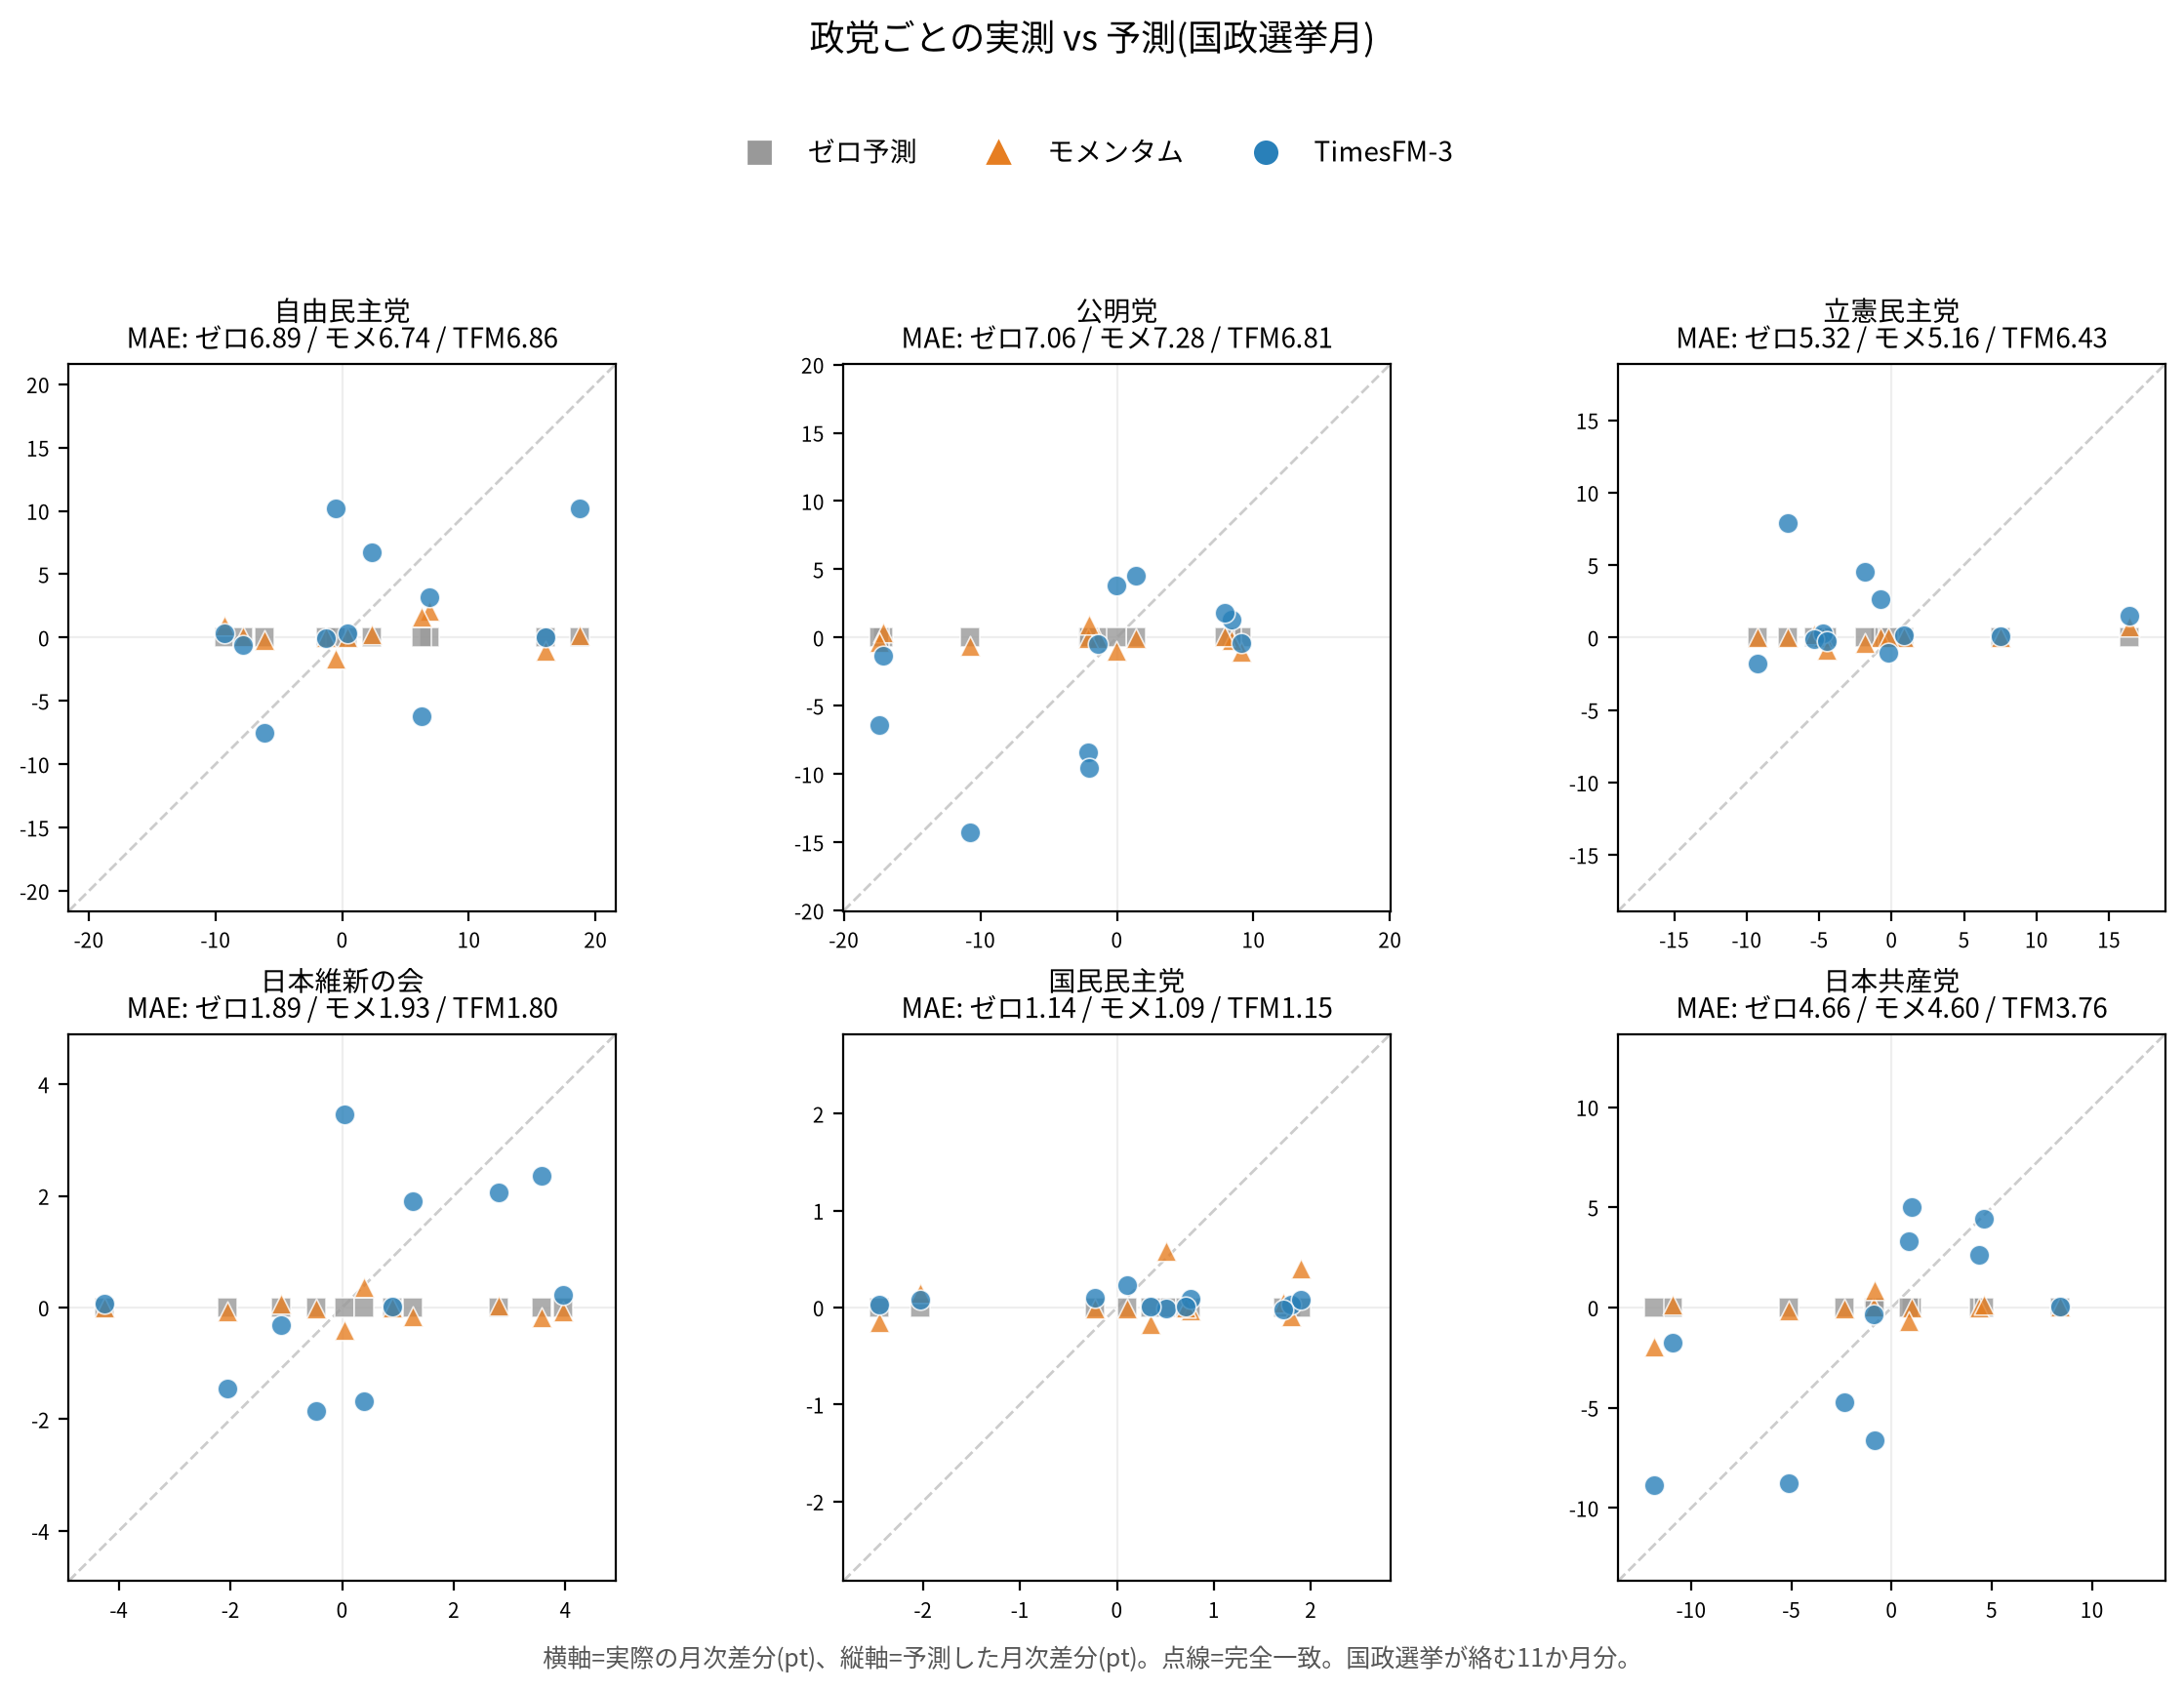
\includegraphics[width=0.9\textwidth]{notes/images/tfm_backtest_scatter_perparty.png}
\caption{政党ごとの実測 vs 予測(国政選挙が絡む11か月、点線は完全一致)}
\label{fig:timesfm-scatter}
\end{figure}

政党ごとに方向的中率の二項検定と順位相関の有意性を確認すると、慣例の両側5\%水準を単独でクリアするのは公明党(順位相関0.68、$p=0.021$)と日本共産党(順位相関0.77、$p=0.006$。方向的中率は11か月全て一致し、二項検定で片側$p=0.0005$、両側$p=0.0010$)の2党だけである。自由民主党(順位相関0.40、$p=0.223$)・日本維新の会(順位相関0.51、$p=0.109$)・立憲民主党(順位相関0.12、$p=0.725$)・国民民主党(順位相関$-0.36$、$p=0.277$)は、いずれも単独では有意水準に届かない。ただし6党について個別に検定しているため多重比較の問題があり、Bonferroni補正後の基準($0.05/6\approx0.0083$)まで考慮すると、日本共産党だけが有意性を維持し、公明党の$p=0.021$は補正後には有意でなくなる。

これは、11か月という標本数が政党単位の検定には少なすぎることが一因だと考えられる。6党×11か月ぶん(n=66)の順位相関をプールすると、TimesFM-3は$\rho=0.503$まで上がり、モメンタム予測の$\rho=0.117$を上回る。ただし6党の値は同じ月の同じ国政選挙という共通の事象を共有しているため、66件を独立試行として扱うナイーブな検定は有意性を過大評価する。そこで、11回の国政選挙イベントを独立な単位とみなし、どのイベントの予測をどのイベントの実測と組み合わせるかをシャッフルするブロック置換検定を行った(20万回のモンテカルロ)。この検定でのTimesFM-3の両側$p$値は0.051、モメンタム予測は0.607である\footnote{選挙イベント単位でブロックを組むことで、同じ月の6党が同じ選挙という共通ショックを共有する非独立性を検定に反映している。}。TimesFM-3は慣例の5\%水準にほぼ届く一方でモメンタムには方向感自体が無いという対比は変わらないが、ナイーブな66件計算の「$p<0.0001$」ほど強い主張はできない。議席規模で最も重要な自由民主党が単独では有意に届かないのは一見奇妙に見えるが、$C_p(T)$は追跡対象の全政党(現在10党)で正規化された相対値であるため、「自民党が伸びるか」を当てることは実質的に「自民党対それ以外の全政党」を当てることと同じ問いになっている。単独検定の非力さがそのまま表れているだけだと考えるのが妥当である。

\textbf{採用ルール}: 政党ごとの有意性で線引きすると、n=11という少ない標本数に基づく事後的な選別になってしまう。そこでプールした検定結果を優先し、covariateが立つ月に限ってバックテスト対象の6党全てにTimesFM-3の予測を使う。covariateが立たない平常月は、ゼロ予測を含むいずれの手法も追加の情報を持たないことが表\ref{tab:timesfm-backtest-quiet}で既に確認されているため、予測自体を行わない。バックテスト対象外の政党も同様に予測しない。したがって「予測」は国政選挙が絡む月にのみ発生するイベントとして扱う。この6党という区切り、およびバックテスト対象外の政党の除外は、いずれも現時点でのデータの蓄積量に基づく暫定的な判断であり、恒久的なものではない。対象政党の国政選挙イベント数が増えるたびに定期的に見直す。

\textbf{採用ルールの予測値が実測と大きく乖離したケースを個別に確認したところ、理由が分かるものと分からないものがあった。} 乖離の大きい上位ケースを実際の政治的な出来事と突き合わせた。

\begin{itemize}
  \item \textbf{理由が分かるもの(2024年10月、公明党・立憲民主党)}: 政治資金問題への批判票が立憲民主党に集まり(実測$+0.164$、予測$+0.015$)、公明党は代表の落選を含む苦戦(実測$-0.174$、予測$-0.064$)をしたことが実際に報じられている月である。TimesFM-3はどちらも方向自体は捉えていたが、動きの大きさまでは予測できなかった。
  \item \textbf{理由が分かるもの(2026年2月、立憲民主党)}: 立憲民主党・公明党の合流で中道改革連合が誕生した月である。政党そのものが実質的に統合された構造変化であり、時系列モデルが予測できる性質のものではない。
  \item \textbf{理由が分かるもの(2025年7月、自由民主党)}: 自民党・公明党で参院過半数割れという、通常は国政選挙が自民党に有利に働く傾向(本節の2024年10月衆院選の分析、野党票の分散効果。実際、6回の実際の国政選挙のうち5回で自由民主党の実測差分は正である)を裏切る異例の結果だった月である(実測$-0.005$、予測$+0.102$)。
  \item \textbf{理由が分かるもの(2024年4月、公明党、covariate対象外の月)}: 国政選挙の無い月にもかかわらず、公明党の実測が$+0.108$動いた。単月の生データを見ると、その月の地方選挙(51件)の中で公明党が18.2\%という異例の強さを見せており、国政選挙のカレンダーとは無関係な地方選挙側の動きだった。
  \item \textbf{理由が分からないもの(2020年7月・2021年10月)}: この2か月は6党とも予測の絶対値が0.02未満とほぼゼロに張り付き、実際の動き(最大で自由民主党$\pm0.16$前後)を取り逃している。バックテストの対象としては初期にあたり、TimesFM-3が参照できる過去の文脈がまだ短かった(12〜44か月)ことが一因である可能性があるが、断定はできない。
  \item \textbf{理由が分からないもの(2026年7月、自由民主党)}: 実測$+0.063$に対し予測は$-0.062$と、符号自体が逆転した。この月は2025年7月参院選が12か月の後方窓から抜けるタイミングにあたるが、なぜ逆方向に外れたのかは特定できていない。単なる大きさの見誤りではなく、方向を外した数少ない例である。
\end{itemize}

以上から、この残差診断は「大勝・大負けの検知」に一定の実用性があるが、残差が大きいこと自体は「国政選挙由来の想定超過」「政党合流のような構造変化」「地方選挙単独の動き」「文脈不足による予測の質の限界」のいずれもあり得るため、機械的に「大勝・大負けだ」と結論せず、単月の生データで裏取りする一手間を記事化のたびに挟む運用とする。

\subsection{「地方選は国政選挙の前哨戦」説の検証}
\label{sec:local-national-precursor}

政治報道でよく語られる「統一地方選のような地方選挙の結果が、後に続く国政選挙の前哨戦になる」という言説を、$C_p(T)$の構成要素を使って検証できないか試みた(2026年9月にユーザー提案)。\texttt{monthly\_index.build\_month\_snapshots()}の内部で使う\texttt{fetch\_sangiin\_election\_history}・\texttt{fetch\_shugiin\_history}を空リストを返すダミーに差し替えるだけで、新規実装なしに「国会の選挙を一切含まない地方選挙限定の$C_p(t)$」を再構成できた。

\textbf{差分(モメンタム)で検証すると、政党ごとに際立って異なる結果になった。} 衆院選・参院選それぞれ連続する回のペア(2019→2022年参院選、2022→2025年参院選、2021→2024年衆院選、2024→2026年衆院選、計4組)について、各党の国政選挙結果の増減方向と、対応する時期の地方限定$C_p$の増減方向が一致するかを見た。プールした一致率は自由民主党を除く5党で70\%(14/20、$\phi=0.39$)だが、二項検定では片側$p=0.058$と慣例の5\%水準に届かない。ところが政党ごとに内訳を見ると、プールした数字からは想像しにくい極端な分布になっている(表\ref{tab:local-momentum})。立憲民主党・国民民主党・日本共産党の3党は4組全てで方向が一致し、日本維新の会は4組全てで方向が逆だった。方向がランダムだと仮定すると、6党のうち4党が「全一致」または「全逆」という極端な結果になる確率は$\binom{6}{4}(2\times0.5^4)^4(1-2\times0.5^4)^2\approx0.30\%$であり、偶然にしては起こりにくい。

\begin{table}[h]
\centering
\small
\caption{政党別の方向一致(国政選挙の連続する回、4組中)}
\label{tab:local-momentum}
\begin{tabular}{lc}
\toprule
政党 & 一致した組数 \\
\midrule
立憲民主党 & 4/4 \\
国民民主党 & 4/4 \\
日本共産党 & 4/4 \\
公明党 & 2/4 \\
自由民主党 & 1/4 \\
日本維新の会 & 0/4 \\
\bottomrule
\end{tabular}
\end{table}

\textbf{この検証から言えることは、意外性を伴う形でこうまとめられる。} 差分で検証すると、プールした一致率(70\%)だけを見れば「五分五分よりましな程度」で終わるところを、政党ごとに割ると6党中4党が偶然では起こりにくい(0.30\%)ほど極端に一致・不一致していることが分かった。ただしこの検証で答え合わせできる独立事象は実質4組しかない。これは日本の国政選挙の頻度そのものに起因する構造的な上限であり、地方側のデータをどれだけ細かく取っても、比較対象の国政選挙が実際に何回行われたかでしか増えない。したがって現時点では、確証ではなく「今後の国政選挙のたびに検証を積み重ねるべき仮説」として記録するにとどめ、次の国政選挙が終わるたびにこの表を更新していく。

\textbf{逆方向、すなわち国政選挙の結果がその後の地方選挙の動きに持ち越されるかも確認した。} 国政選挙イベント月の直後1か月の実測差分は、他の平常月と比べて平均に有意差が無く(6党いずれも$p>0.09$)、イベント月自体の実測差分と翌月の実測差分の相関も6党いずれも有意ではない($p>0.24$)。少なくとも1か月先までは、国政選挙の勢いが地方選挙側に持ち越される効果は検出できなかった。

\textbf{以上を総合すると、地方選挙は国政選挙の縮図ではなく、ほぼ独立に動いているという描像になる。} 国政選挙が絡まない月の$C_p(T)$はランダムウォークに近く(\ref{sec:timesfm-backtest}節)、国政選挙の結果が翌月以降の地方選挙に持ち越された形跡もない。唯一残るのは逆方向、すなわち地方選挙の勢いの変化の\textbf{方向}が次の国政選挙の結果の方向とある程度対応するという弱い証拠であり、これも大きさの対応までは確認できていない。「地方選は国政選挙の前哨戦」という通説は、方向に限れば部分的に裏付けられる。ただし今回検証したのはあくまで方向であり、地方の動きの規模から国政選挙の結果の規模まで読み取れるかどうかは検証していない。

\section{免責事項・データ出典}

本プロジェクトは個人による非公式の集計であり、政府・政党・報道機関等が公式に発表するものではありません。算出結果には集計方法・データ取得時点に起因する誤差、実装上の不具合による誤りが含まれる可能性があります。本資料・算出コード・算出結果は現状有姿で提供され、内容の正確性・完全性を保証しません。政治的な意思決定や公式な議論の根拠として利用する際は、必ず一次資料(表\ref{tab:datasource-recap}および\S4のデータソース節に記載の各URL)にあたって確認してください。

\begin{table}[h]
\centering
\caption{主要データの出典(詳細は\S4参照)}
\label{tab:datasource-recap}
\begin{tabular}{p{9.5cm}p{5.0cm}}
\toprule
データ種別 & 出典機関 \\
\midrule
国会の議席 & 衆議院・参議院(各院公式サイト) \\
地方議会・首長の議席 & 総務省 \\
国・地方の予算 & 財務省、総務省 \\
首長の推薦・支持政党 & 公益財団法人地方自治総合研究所「全国首長名簿」 \\
市区町村コードの変遷 & 総務省 \\
知事の議席台帳の直近値(補完) & 政治山(非公式・民間サイト) \\
市区町村長・地方議会の議席台帳の直近値(補完) & 選挙ドットコム(非公式・民間サイト) \\
市区町村長の直近値(選挙ドットコムで取得できない場合の補完) & Wikidata \\
\bottomrule
\end{tabular}
\end{table}

本プロジェクトの指数設計・データソース調査・実装にはAI(Claude)を活用しています。詳細は\S1.2を参照してください。

\subsection{ライセンス}

算出コード(リポジトリの\texttt{src/}以下)はMIT Licenseで公開します。本設計書・READMEの説明文・note記事等の文章については著作権を放棄していません。

\end{document}
